\PassOptionsToPackage{table,xcdraw}{xcolor} %DIF > 
\documentclass[11pt]{article}
\usepackage{graphicx} % Required for inserting images
% \usepackage{amsmath}
\usepackage{lipsum}
\usepackage{pdfcomment}

\usepackage{tikz}
\usepackage{caption}
\usepackage{amsmath}
\usetikzlibrary{positioning}
\usetikzlibrary{arrows.meta, positioning}

\usepackage{xcolor} % Enable table colors and HTML color codes %DIF > 
\usepackage{subcaption}
% \usepackage[english]{babel}
% \usepackage[utf8]{inputenc}
% \usepackage{amsfonts}
\usepackage{longtable}
\usepackage{graphicx}
\usepackage{float}
\usepackage{booktabs}
\usepackage{float} 
\usepackage{geometry}
\usepackage{lineno}
\usepackage{authblk}
\usepackage{tcolorbox}
\usepackage{rotating}
\usepackage{booktabs}
\usepackage{threeparttable}
\usepackage{geometry} % Optional: for full page layout control
%margin
\geometry{
    left=1in,
    right=1in,
    top=1in,
    bottom=1in
}

\usepackage{lscape}
\usepackage{siunitx}  % For aligning numbers on the decimal point
\usepackage{adjustbox} % To adjust table width if needed
\usepackage{pgfplots}
\usepackage{caption}
\usepgfplotslibrary{groupplots}

% Use natbib with sort&compress
\usepackage[numbers,sort&compress]{natbib}

\usepackage{hyperref}
\hypersetup{
  colorlinks=true,
  linkcolor=blue,       % 章节跳转链接（如目录、交叉引用）
  citecolor=blue,       % 文献引用
  urlcolor=blue         % 网页链接
}

\usepackage{cite}

%font type and line spacing
% \usepackage{mathpazo}
\renewcommand{\baselinestretch}{1.5}

% \renewcommand{\arraystretch}{0.5} % 数字 <1 压缩, >1 拉伸

\usepackage{array}
\usepackage{multirow}

\usepackage{amssymb}
\usepackage{pifont}

\usepackage[colorinlistoftodos]{todonotes}

% \usepackage{times}

%chinese
% \usepackage{xeCJK}

\usepackage{wrapfig}

%remove all paragraph indent
% \usepackage{parskip}

% Use BibTeX for bibliography management (uncomment this if author name is needed.
% \usepackage[semicolon]{natbib}
% \usepackage[numbers,sort]{natbib}
\usepackage{cite}

%margin
\geometry{
    left=1in,
    right=1in,
    top=1in,
    bottom=1in
}

% \hypersetup{
%     colorlinks=true, % Enable colored links
%     linkcolor=black,  % Set the color of internal links (e.g., references)
%     citecolor=blue, % Change this color as desired
%     urlcolor=blue    % Set the color of external links (e.g., URLs)
% }

\usepackage{amsthm}
\newtheorem{example}{Example}[section] % Define the example environment
\newtheorem{homework}{Homework} % Define the example environment

\renewcommand\Authfont{\normalsize} % 作者名正常大小+加粗
\renewcommand\Affilfont{\small\normalfont}   % 单位小一号

\usepackage{titlesec}
\usepackage{titletoc}
% Define \subsubsubsection
\titleclass{\subsubsubsection}{straight}[\subsection]
\newcounter{subsubsubsection}[subsubsection]
\renewcommand\thesubsubsubsection{\thesubsubsection.\arabic{subsubsubsection}}
\titleformat{\subsubsubsection}{\normalfont\normalsize\bfseries}{\thesubsubsubsection}{1em}{}
\titlespacing*{\subsubsubsection}{0pt}{3.25ex plus 1ex minus .2ex}{1.5ex plus .2ex}
\setcounter{secnumdepth}{4} % Numbering depth
\setcounter{tocdepth}{4} % Include subsubsubsections in the table of contents

% % Set section headings to 10pt
\titleformat*{\section}{\fontsize{11}{12}\selectfont\bfseries}
\titleformat*{\subsection}{\fontsize{11}{12}\selectfont\bfseries}
\titleformat*{\subsubsection}{\fontsize{11}{12}\selectfont\bfseries}
\titleformat*{\paragraph}{\fontsize{11}{12}\selectfont\bfseries}
\titleformat*{\subparagraph}{\fontsize{11}{12}\selectfont\bfseries}

% Adjust the formatting in the table of contents
\titlecontents{subsubsubsection}
[8em] % adjust this value to fit your needs
{\small}
{\hyperlink{toc.\thecontentslabel}{\thecontentslabel.} }
{}
{\ \titlerule*[.5pc]{.}\contentspage}

\titlespacing*{\subsubsubsection}{0pt}{3.25ex plus 1ex minus .2ex}{1.5ex plus .2ex}

\usepackage{caption}
% Make the label bold and keep the caption text regular
\captionsetup{
  labelfont=bf, % makes label (e.g., "Figure 1") bold
  textfont=small % keeps caption text in normal font
}

% \usepackage{sectsty}
% % Remove indentation after section headings
% \sectionfont{\noindent}

%remove hyphenation
\usepackage{microtype}

\usepackage{enumitem}
% Set item separation globally
\setlist{itemsep=0em}

% % Adjust the space after figure captions
% \setlength{\belowcaptionskip}{-15pt}

\usepackage{fancyhdr} % For custom headers/footers
\usepackage{lastpage} % For total number of pages

\pagestyle{fancy}
\fancyhf{} % Clear header/footer
\fancyfoot[C]{\thepage\ of \pageref{LastPage}} % Page number as x out of total
\renewcommand{\headrulewidth}{0pt} % Remove horizontal line from header

\usepackage{listings}

\definecolor{codegreen}{rgb}{0,0.6,0}
\definecolor{codegray}{rgb}{0.5,0.5,0.5}
\definecolor{codepurple}{rgb}{0.58,0,0.82}
\definecolor{backcolour}{rgb}{0.95,0.95,0.92}

\lstdefinestyle{mystyle}{
    backgroundcolor=\color{backcolour},   
    commentstyle=\color{codegreen},
    keywordstyle=\color{magenta},
    numberstyle=\tiny\color{codegray},
    stringstyle=\color{codepurple},
    basicstyle=\ttfamily\footnotesize,
    breakatwhitespace=false,         
    breaklines=true,                 
    captionpos=b,                    
    keepspaces=true,                 
    numbers=left,                    
    numbersep=5pt,                  
    showspaces=false,                
    showstringspaces=false,
    showtabs=false,                  
    tabsize=2
}

\lstset{style=mystyle}

\title{Ergonomic Risk Detection and Mitigation Using YOLOv8 with Vision-Language Models and Retrieval-Augmented Generation}

% \author[1]{Sarayu Varma Gottimukkala}
% \author[1]{Lu Gao, Ph.D. \thanks{lgao5@central.uh.edu}}
% \author[1]{Zia Din, Ph.D.}
% \author[1]{Kinam Kim, Ph.D.}
% \author[2]{Jingran Sun, Ph.D.}
% \affil[1]{Department of Civil and Environmental Engineering, University of Houston}
% \affil[2]{Department of Civil and Environmental Engineering, University of South Florida}
\author{}
\date{}
\providecommand{\DIFadd}[1]{#1}
\providecommand{\DIFdel}[1]{}
\providecommand{\DIFaddFL}[1]{#1}
\providecommand{\DIFdelFL}[1]{}
\providecommand{\DIFaddbegin}{}
\providecommand{\DIFaddend}{}
\providecommand{\DIFaddbeginFL}{}
\providecommand{\DIFaddendFL}{}
\providecommand{\DIFdelbegin}{}
\providecommand{\DIFdelend}{}
\providecommand{\DIFdelbeginFL}{}
\providecommand{\DIFdelendFL}{}
\begin{document}

\linenumbers % 开启行号

\maketitle    

\begin{abstract}
Work-related injuries remains a significant and ongoing concern in the construction industry. This research presents a computer-vision based approach for detecting and assessing ergonomic risks among construction workers. The system performs five key functions: (1) assessment of workers' postures; (2) identification of normal and risky physical activities; (3) measurement of activity duration; (4) quantification of high-risk movement frequency; (5) recommendations for risk mitigation using Large Language Models. To validate its performance, the system was tested on video datasets capturing various construction tasks such as drywall finishing, hand screeding, kneeling finishing, laying concrete blocks, and tying rebar. Results were benchmarked against expert annotated groud truth data, which demonstrated high accuracy in detecting ergonomic risks. Overall accuracy exceeded 90\% across multiple task categories, which confirms the reliability of the system in detecting both postures and activity transitions. The proposed approach allows construction managers to identify unsafe practices on-site.
\end{abstract}

\noindent \textbf{Keywords:} Ergonomic Risk, Construction Worker, Computer Vision, Vision Language Model, Retrieval-Augmented Generation

% \end{abstract}
%
%
%

\newpage
\section{Introduction}

It is reported that the prevalence of work-related injuries among construction workers reached 34\% in the US in 2020 \citep{antwi2020construction}. These risks in construction arise from physical, environmental, and organizational factors. Physical demands such as heavy lifting, repetitive movements, prolonged static postures, and awkward positions increase injuries like low back pain and joint disorders \citep{singh2024construction}. Environmental conditions, including slippery surfaces, poor lighting, extreme temperatures, and disorganized worksites, force unsafe positions and raise physical strain \citep{ishwarya2021analysis}. Organizational issues such as insufficient training, lack of rest breaks, heavy workloads, and poor supervision further amplify risks by pushing workers beyond their physical limits \citep{mohan2018identifying}. Given the complex and multifactorial nature of ergonomic risks, efficient monitoring and real-time feedback systems are urgently needed.

Computer vision methods are increasingly being used to automate ergonomic risk detection by analyzing workers' postures and movements through cameras and algorithms \citep{seo2021automated}. A typical workflow involves applying deep learning and computer vision models to identify key body parts, such as the head, knees, and shoulders, in images captured on construction sites. These identified points are used to construct a skeletal representation of the worker. From this skeletal structure, joint positions are determined, which allows for the calculation of joint angles. These joint angles are then used to assess ergonomic risk using established metrics such as the Ovako Working Posture Analysis System (OWAS) \citep{karhu1977correcting}, Rapid Upper Limb Assessment (RULA) \citep{mcatamney1993rula}, and Rapid Entire Body Assessment (REBA) \citep{hignett2000rapid}. These assessment tools classify specific worker postures into different levels of injury risk.

However, current computer vision and posture estimation methods for ergonomic risk detection face several limitations in real-world construction environments. These include   a predominant focus on single-frame posture recognition while neglecting temporal  factors such as repetition and   duration, as well as a lack of mechanisms for delivering corrective feedback after a risk is identified . To address these issues, this research developed a n  ergonomic risk detection system   that analyzes construction workers' postures and provides  actionable feedback to help mitigate musculoskeletal disorders. The   main  contributions of this study are   summarized as follows:

\begin{enumerate}[nosep, leftmargin=*]
    \item A vision-based pipeline using the \textit{yolov8n-pose} model to detect worker keypoints and estimate posture from construction site videos.
    \item A temporal analysis module that tracks bending duration, bending transitions, and trunk-flexion-based REBA scoring across consecutive frames rather than relying only on isolated images.
    \item A full workflow for identifying ergonomically risky activities in multiple construction tasks using automated pose estimation, tracking, and activity segmentation.
    \item A vision-language-model-assisted component that identifies handled tools or objects and supports approximate REBA load-category interpretation, together with a  retrieval-augmented   recommendation module for context-aware ergonomic risk mitigation guidance.
\end{enumerate}
 

  To improve the overall clarity of the workflow, Figure~\ref{fig:graphical_abstract} provides a graphical abstract of the complete system presented in this paper. It summarizes how construction video frames are processed through pose estimation and tracking, full-body REBA scoring, temporal activity analysis, and the VLM--RAG recommendation module to produce ergonomic risk indicators and mitigation guidance.

\begin{figure}[H]
\centering
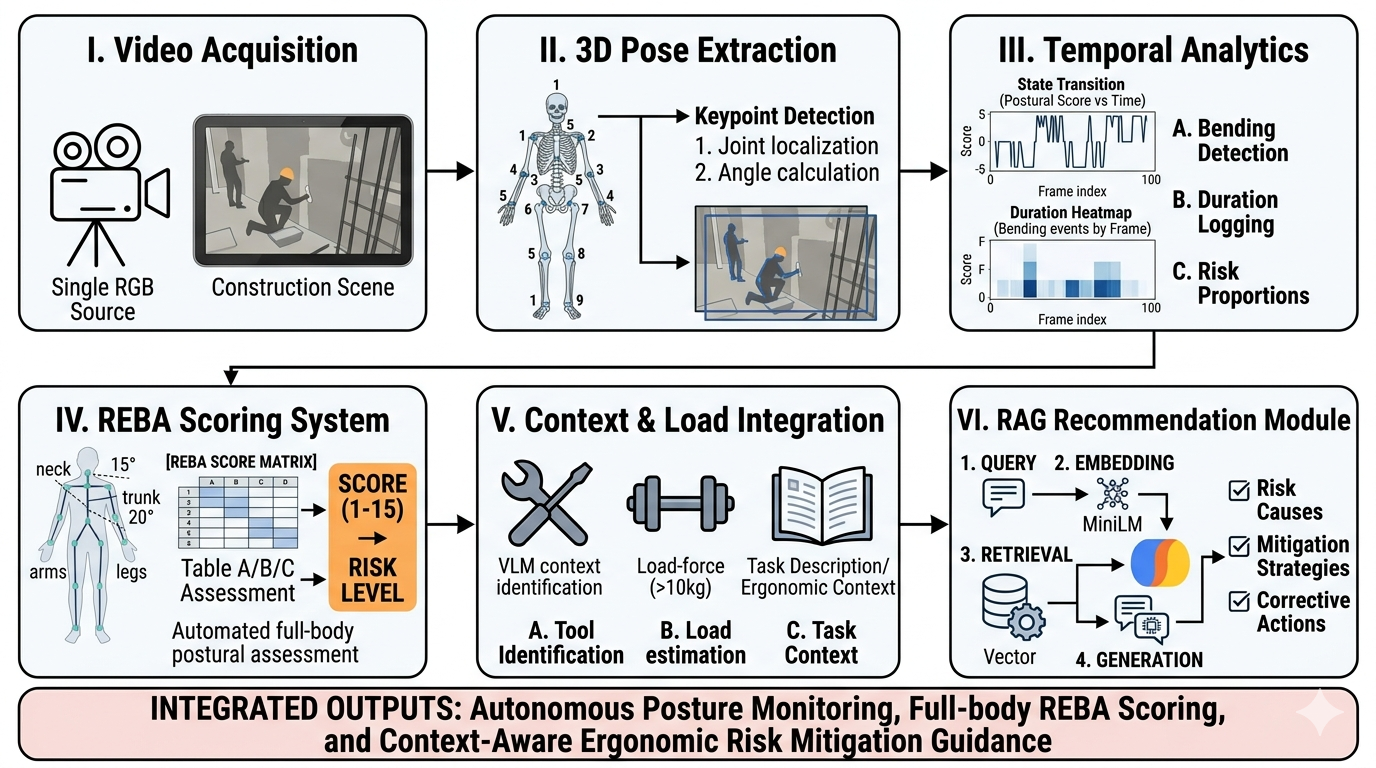
\includegraphics[width=\textwidth]{figures/graphical_abstract_workflow_gemini.png}
\caption{Graphical abstract of the proposed framework. Construction site video is processed through YOLOv8 pose detection, temporal tracking, full-body REBA computation, VLM-assisted approximate load interpretation, and a retrieval-augmented recommendation module to generate ergonomic risk scores, temporal exposure measures, and mitigation guidance.}
\label{fig:graphical_abstract}
\end{figure}

  The remainder of this paper is organized as follows: Section 2 presents a comprehensive literature review covering ergonomic risks in construction, existing assessment methods, and computer vision applications. Section 3 details the proposed methodology, including system architecture, pose estimation techniques, and risk detection algorithms. Section 4 describes the case study implementation and validation results across various construction tasks. Section 5 discuses the findings, limitations, and implications of the research. 

\section{Literature Review}

 Construction work is   \DIFadd{physically demanding and frequently requires repetitive motions, awkward postures, kneeling, stooping, and material handling under dynamic site conditions \mbox{%DIFAUXCMD
\citep{inyang2012ergonomic}}\hskip0pt%DIFAUXCMD
. As a result, } musculoskeletal disorders  remain a persistent concern in the industry. Prior studies have reported high prevalence rates of musculoskeletal symptoms  among construction workers   \DIFadd{across multiple countries, which highlights the need for scalable and objective ergonomic monitoring methods \mbox{%DIFAUXCMD
\citep{massirisfernandez2020ergonomic,chen2024automatic}}\hskip0pt%DIFAUXCMD
. Common mitigation strategies include ergonomic } job design,  engineering controls,   work-practice  controls, administrative   interventions , and early identification of   hazardous  postures and movements  \citep{antwi2018wearable}.

  Ergonomic assessment approaches can generally be grouped into  self-report , observation-based  \DIFadd{, and direct-measurement methods \mbox{%DIFAUXCMD
\citep{tao2024evaluation}}\hskip0pt%DIFAUXCMD
. } Self-report   tools such as  the Nordic Musculoskeletal Questionnaire  and the Borg   \DIFadd{scale capture workers' perceived discomfort and exertion, but they do not directly measure posture or external exposure \mbox{%DIFAUXCMD
\citep{kuorinka1987standardised,borg1982psychophysical}}\hskip0pt%DIFAUXCMD
. } Observation-based methods   including  OWAS, RULA, and REBA   \DIFadd{provide structured frameworks for rating posture-related risk, yet manual scoring is time consuming and subject to human variability \mbox{%DIFAUXCMD
\citep{karhu1977correcting,mcatamney1993rula,hignett2000rapid,zhang2017real}}\hskip0pt%DIFAUXCMD
. Direct-measurement approaches using motion capture} , inertial measurement units, pressure insoles, and electromyography   can provide continuous quantitative data ,  but they often require specialized hardware, increase deployment cost,  and may interfere with   \DIFadd{worker activity \mbox{%DIFAUXCMD
\citep{mudiyanselage2021automated,zhao2018health,li2024data}}\hskip0pt%DIFAUXCMD
} .

  Computer vision research has attempted to address these limitations by automating posture recognition from images and video. Earlier methods  relied on 2D   \DIFadd{image features and conventional classifiers \mbox{%DIFAUXCMD
\citep{yan2017development,seo2021automated}}\hskip0pt%DIFAUXCMD
. More recent approaches use deep learning, } 3D pose estimation  \DIFadd{, and automated ergonomic scoring. For example, \mbox{%DIFAUXCMD
\citet{yu2019joint} }\hskip0pt%DIFAUXCMD
integrated } 3D   \DIFadd{pose estimation with REBA, \mbox{%DIFAUXCMD
\citet{massirisfernandez2020ergonomic} }\hskip0pt%DIFAUXCMD
computed RULA scores from image data } under real working conditions  \DIFadd{, and \mbox{%DIFAUXCMD
\citet{li2024data} }\hskip0pt%DIFAUXCMD
combined } 3D   RGB-based pose estimation with a data-driven inference framework. Temporal modeling has also begun to appear in the literature through approaches such as recurrent models for posture recognition and  transformer-based   \DIFadd{repetitive action counting \mbox{%DIFAUXCMD
\citep{zhao2021applying,wang20233d,chen2024automatic}}\hskip0pt%DIFAUXCMD
. However, most prior studies still emphasize posture recognition or scoring at the frame level. In contrast, the present work combines pose estimation with temporal bending-frequency tracking, posture-duration measurement,   }full-body REBA scoring, VLM-assisted approximate load estimation,  and retrieval-augmented LLM feedback so that detected risks can be interpreted and acted upon within a single workflow .

\section{Methodology}
% \subsection{System Design and Architecture}

To enable real-time, low-cost ergonomic risk monitoring in dynamic construction environments, we design a lightweight system deployable with a single RGB camera and an edge device. It comprises a camera that captures video feeds of workers during routine activities. The stream is processed in real time by   the \textit{yolov8n-pose} model  to identify each worker and estimate their pose. Capture, processing, and visualization are implemented with OpenCV. The architecture includes modules for pose estimation, activity monitoring, and risk analysis. Figure \ref{fig1} presents the system architecture for human pose detection. 

% The ergonomic risk detection system is designed using the YOLOv8 architecture \citep{terven2023comprehensive}. The system begins with an input image resized to dimensions of 640×640×3 and processes it through three primary stages: backbone, neck, and head. The backbone is responsible for extracting key features from the input image. It uses CBS modules (Convolution, Batch Normalization, and SiLU activation layers) to enhance the image features by detecting essential patterns like edges, shapes, and textures. To capture a wide range of details, C2F (Cascaded Convolution with different Filter sizes) modules are applied. C2F focuses on both broad patterns, such as body shapes, and finer details, such as the positions of hands or feet. Stride-2 convolutions are used to reduce the spatial size of the image. Later, up-sampling steps restore the resolution, which ensures that no essential features are lost.

 \subsection{YOLOv8 Pose Estimation Pipeline}

 The ergonomic risk detection system is designed   \DIFadd{around the YOLO family of one-stage detectors. We cite both the original YOLO formulation by \mbox{%DIFAUXCMD
\citet{redmon2016yolo} }\hskip0pt%DIFAUXCMD
and the later architectural review by \mbox{%DIFAUXCMD
\citet{terven2023comprehensive}}\hskip0pt%DIFAUXCMD
; the specific pose model used in this study is }\textit{yolov8n-pose}. In this paper, the terms ``backbone,'' ``neck,'' and ``head'' refer to standard stages of the detection network architecture rather than anatomical regions of the worker. The backbone extracts image features, the neck fuses features across scales, and the head predicts person bounding boxes and body keypoints.

The input image is  resized to 640×640×3 and   processed through these three stages. In the backbone,  CBS modules (convolution, batch normalization, and SiLU   activation) extract low- and mid-level visual features.  C2f blocks  \DIFadd{, which are derived from cross-stage-partial feature reuse principles, improve gradient flow and computation efficiency \mbox{%DIFAUXCMD
\citep{wang2020cspnet}}\hskip0pt%DIFAUXCMD
. An SPPF block near } the end of the backbone aggregates multiscale   \DIFadd{spatial context \mbox{%DIFAUXCMD
\citep{he2015spatial}}\hskip0pt%DIFAUXCMD
. The neck performs multiscale fusion using } a feature pyramid   and  path aggregation, commonly   \DIFadd{described through the FPN and PAN structures \mbox{%DIFAUXCMD
\citep{lin2017fpn,liu2018panet}}\hskip0pt%DIFAUXCMD
. Finally, the decoupled anchor-free head predicts one person bounding box and a set of body keypoints for each detected instance.
}

A minimum keypoint confidence threshold of  0.5   was selected after empirical tuning to balance false positives and missed detections. Keypoints whose confidence falls below this threshold are treated as undetected for that frame and are not passed directly to the downstream posture-analysis module.
YOLOv8 was selected for the present study because it provides person detection and pose estimation within a single lightweight pipeline that is suitable for near-real-time deployment on ordinary hardware. More specialized pose-estimation toolkits and video-based methods, including RTMPose, MMPose, and VideoPose3D-style temporal reconstruction pipelines, are valuable comparison targets for future work. However, the current benchmark focused on comparing the proposed YOLOv8 variants against an established baseline implementation of OpenPose under the same construction clips and downstream REBA workflow.
 % Thresholds below 0.5 caused the model to mistakenly identify joints on non-human objects and reduced the clarity of human posture detection. Conversely, thresholds above 0.5 were overly strict and filtered out some actual human detections and leading to incomplete posture analysis. 
Additionally, smoothing techniques are used to stabilize the detected keypoints across frames, which prevents jitter in real-time applications.

% The final output of the system is a skeletal overlay on the original image, visually representing the detected poses and body keypoints. This design is highly effective for applications such as construction safety monitoring, where it is important to evaluate workers’ postures and identify risky positions or movements that could lead to injuries. By providing accurate feedback in real time, the system helps prevent workplace accidents and ensures ergonomic safety in dynamic environments.

\begin{figure}[H]
\centering
\begin{subfigure}[b]{0.9\textwidth}
    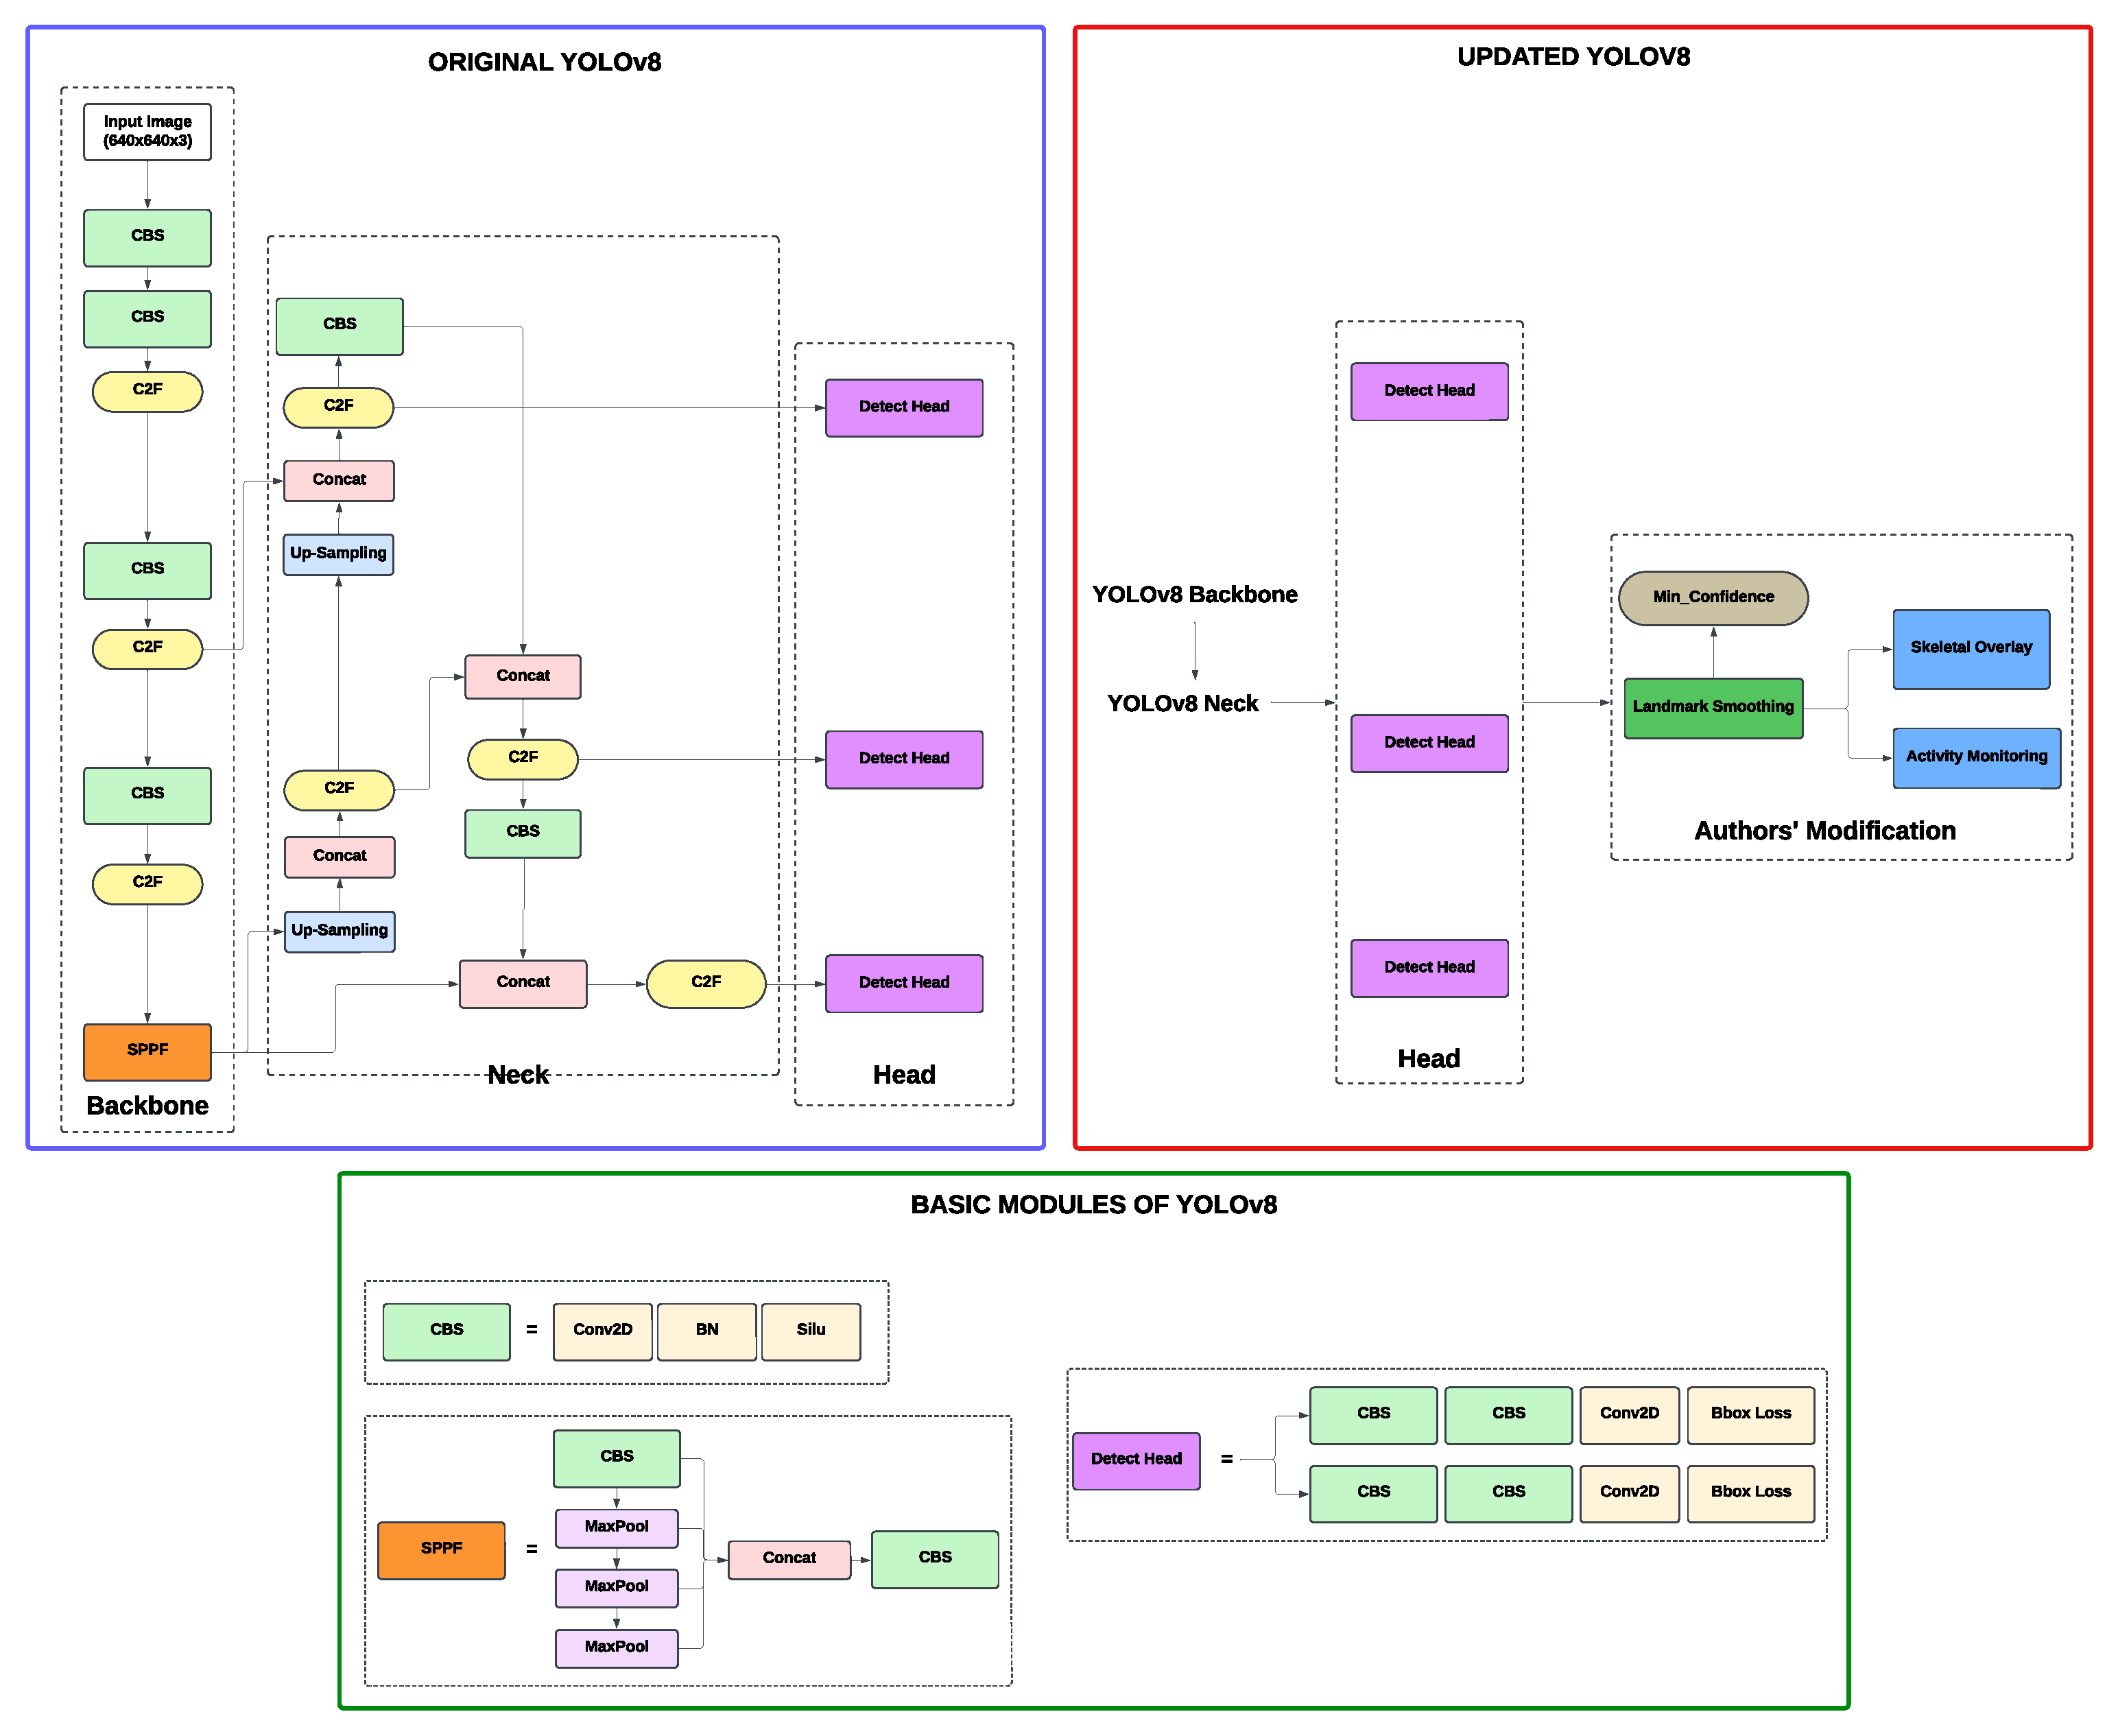
\includegraphics[width=\textwidth]{figures/Methodology.pdf}
    \end{subfigure}
    \caption{Proposed Architecture} 
    \label{fig1}
\end{figure}

\subsection{Pose Estimation and Landmark Smoothing}
Pose estimation in this approach relies on   \textit{yolov8n-pose}  to estimate body keypoints for worker posture assessment: head, shoulders, hips, knees, and ankles. Figure \ref{fig2} represents the various keypoints of the human body that are identified by the YOLOv8 model. The model identifies these keypoints and makes connections between various poses to create a skeleton of the person detected.

\begin{figure}[H]
    \centering
    % \begin{subfigure}[b]{1\textwidth}
    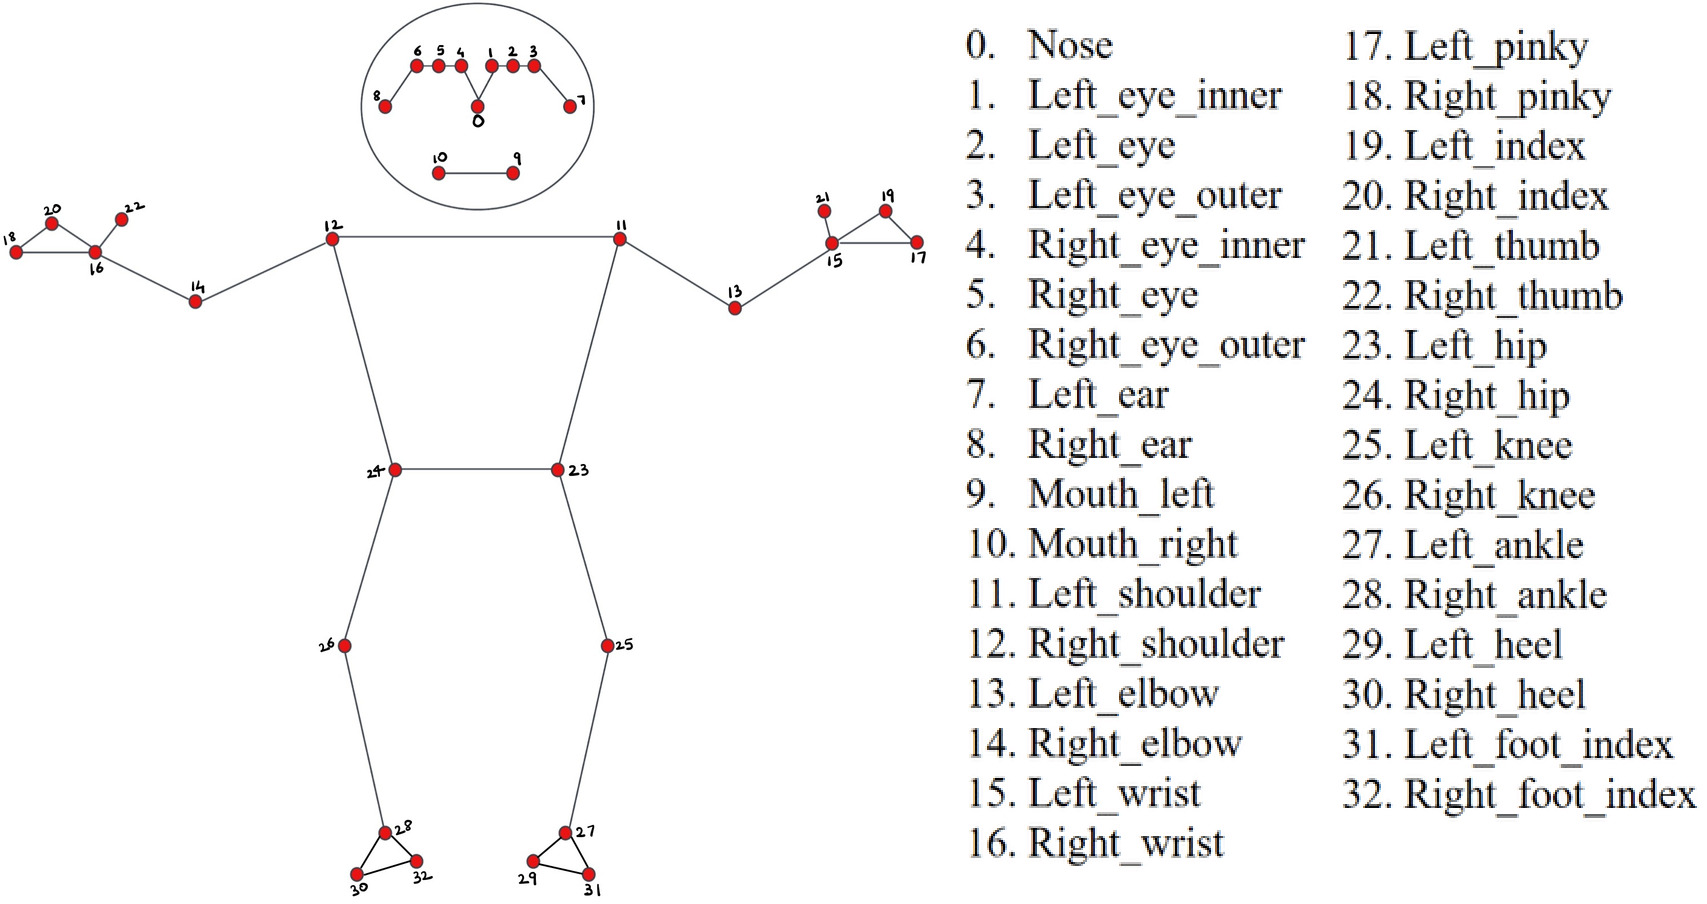
\includegraphics[width=0.5\textwidth]{figures/Poses.jpg}
    % \end{subfigure}
    \caption{Keypoints identified by YOLOv8 model}
    \label{fig2}
\end{figure}

A landmark smoothing technique is performed to increase the stability of the predicted keypoints. The moving average is computed over successive frames for each keypoint  to reduce jitter   and suppress short-lived missing detections. In practice, when a keypoint confidence falls below the minimum threshold, the corresponding output coordinate may collapse to the image origin \((0,0)\). For that reason, the smoothing function acts not only as a jitter filter but also as a lightweight interpolation mechanism that prevents these origin artifacts from propagating directly into downstream posture calculations.  A simple moving average was selected over more complex filtering methods due to its computational efficiency and ease of implementation, which are critical for real-time applications.
% This approach requires minimal parameter tuning. The moving average provided an effective and practical solution without the overhead of more sophisticated filters. 
The landmark smoothing scheme significantly improves the coherence of posture detections, particularly in challenging conditions where rapid movements may introduce noise in the detection process.   The smoothing function averages each keypoint position across successive frames to improve  stability and coherence   in  pose estimation. The  formula used to calculate and incorporate the landmark smoothing mechanism is

\begin{equation}
     S_i = (1 - \alpha)P_i + \alpha C_i
\end{equation}

where, 
\\ $S_i$ = Smoothed coordinates (x,y) of landmark i after smoothing
\\ $P_i$ = (x,y) coordinates of the landmark in previous frame
\\ $C_i$ = (x,y) coordinates of the landmark in current frame
\\ $\alpha$ = Smoothing factor

The smoothing factor reduces jitter in detected keypoints across frames by averaging the current frame’s coordinates with previous frames. It does not   change the confidence-based acceptance rule, but it does alter how accepted  keypoints are positioned and stabilized over time. A smoothing factor of 0.5 was chosen to achieve a balanced trade-off between responsiveness and stability in keypoint tracking. Lower values made the output overly sluggish, which caused delays in reflecting quick posture changes. Higher values introduced instability by allowing too much jitter from rapid movements. A value of 0.5 provided sufficiently smooth trajectories without sacrificing the system’s ability to capture real-time posture dynamics accurately. 

\subsection{  Multi-frame Tracking and  Activity   Segmentation }
  Because ergonomic risk assessment in video requires temporal continuity, detections belonging to the same worker must be associated across frames. We therefore use a centroid-based tracker in which each detected person bounding box is represented by its centroid, and each centroid in the current frame is matched to the nearest centroid from the previous frame within a fixed pixel-distance threshold. This lightweight association step provides persistent person IDs for posture-duration measurement and bending-frequency tracking while remaining suitable for real-time processing.

The tracker also defines how activity segments begin and end. When a worker remains matched across consecutive frames, the same ID is preserved and the standing or bending state is updated continuously. When a worker leaves the field of view and no valid match is found, the active segment is closed at the last valid frame. If that worker later reappears, the new detection is treated as a new tracking segment rather than a continuation of the previous one. This behavior avoids assigning unsupported durations through periods of non-visibility, but it also means that posture duration can be underestimated when workers move out of frame, which is a limitation of the current single-camera implementation.

\subsection{Ergonomically Risky Activity Detection}
This module classifies worker activities using pose landmarks and evaluates ergonomic risk   \DIFadd{using the full REBA framework \mbox{%DIFAUXCMD
\citep{hignett2000rapid}}\hskip0pt%DIFAUXCMD
. The system first detects body keypoints using YOLO pose and then computes posture angles for the neck, trunk, upper arms, lower arms, wrists, and legs from smoothed } 2D   keypoint coordinates. These segment angles are converted into REBA segment scores, combined through REBA Table A, Table B, and Table C, adjusted with a load/force score, and finally mapped to the corresponding REBA risk level. In this way,  the   reported metric is a full REBA score rather than a trunk-only proxy.

Joint angles are derived from vectors formed by adjacent body landmarks. For any two vectors \(\vec{u}\) and \(\vec{v}\), the included angle is calculated using the dot-product relation
\begin{equation}
    \DIFadd{\DIFadd{\theta = \arccos \Bigl( \frac{\vec{u}\cdot\vec{v}}{\|\vec{u}\| \|\vec{v}\|} \Bigr)\times \frac{180}{\pi}.
}}\end{equation}
Trunk flexion is computed from the hip-midpoint to shoulder-midpoint vector against the vertical reference; neck flexion is estimated from the shoulder-midpoint to head vector against the trunk vector; upper-arm angle is measured between the upper arm and trunk; lower-arm angle is measured between the upper-arm and forearm vectors; wrist posture is estimated from the forearm-to-hand configuration; and leg posture is determined from knee flexion and lower-limb support geometry.

The resulting angles are converted into REBA segment scores using the standard rule structure: trunk posture is scored from neutral to severe flexion, neck posture is scored from neutral to flexed posture, upper-arm posture is scored across increasing elevation ranges, lower-arm posture is scored according to deviation from the mid-range elbow position, wrist posture is scored by wrist deviation, and the legs are scored from stable bilateral support to bent or kneeling postures. Trunk, neck, and leg scores are combined through REBA Table A to obtain Score A. Upper-arm, lower-arm, and wrist scores are combined through REBA Table B to obtain Score B. Score A and Score B are then merged through REBA Table C to produce the final REBA score.

For handled tools or materials visible in the frame, a vision-language model is used to identify the object category and support approximate load/force estimation based on typical weight ranges of common construction tools and materials. This estimated load score is then incorporated into the REBA scoring workflow. Coupling is treated as a neutral default when it cannot be inferred reliably from the image  .
 

Let \(\vec{HS}\) be the vector from the hip midpoint \((H_x, H_y)\) to the shoulder midpoint \((S_x, S_y)\), and let \(\vec{V}\) be the vertical reference vector. We define:
\begin{align}
    \vec{HS} & = (S_x - H_x,\; S_y - H_y)\\
    \vec{V} & = (0,\; 1)
\end{align}  

\noindent The trunk angle \(\theta_{\text{trunk}}\) is computed as follows:

\begin{equation}
    \theta_{\text{trunk}} 
    = \arccos \Bigl( \frac{\vec{HS} \cdot \vec{V}}{\|\vec{HS}\|\|\vec{V}\|} \Bigr)
    \times \frac{180}{\pi},
\end{equation}

\noindent where \(\theta_{\text{trunk}}\) is measured in degrees.     Table~\ref{table:reba_segments} summarizes the segment-level REBA rules implemented in the revised system .
 

\begin{table}[H]
\renewcommand{\baselinestretch}{1.0}\selectfont % 只在本表内恢复正常行距
\renewcommand{\arraystretch}{0.92}              % 微调行高
\setlength{\tabcolsep}{4pt}                     % 压缩左右内边距，默认 6pt
\centering
\small
\caption{Implemented REBA segment scoring rules}
\begin{tabular}{l|p{4.9cm}|c}
\hline
\textbf{Segment} & \textbf{Rule} & \textbf{REBA Score} \\
\hline
Trunk & $<5^\circ$, $5^\circ$--$20^\circ$, $20^\circ$--$60^\circ$, $>60^\circ$ & 1, 2, 3, 4 \\
Neck & $\leq 20^\circ$, $>20^\circ$ & 1, 2 \\
Upper arm & $<20^\circ$, $20^\circ$--$45^\circ$, $45^\circ$--$90^\circ$, $>90^\circ$ & 1, 2, 3, 4 \\
Lower arm & $60^\circ$--$100^\circ$, otherwise & 1, 2 \\
Wrist & within $\pm 15^\circ$, otherwise & 1, 2 \\
Legs & stable support, bent/unstable, kneeling/deep flexion & 1, 2--4 \\
\hline
\end{tabular}
    \label{table:reba_segments}
  \end{table}

In this research, a posture is classified as bending when the trunk angle \(\theta_{\text{trunk}}\) exceeds a specified lower threshold (e.g., $20^\circ$).
% More specifically:
% \begin{equation}
%     B = 
%     \begin{cases}
%     1, & \text{if } \theta_{\text{trunk}} \geq 20^\circ,\\
%     0, & \text{otherwise.}
%     \end{cases}
% \end{equation}
Depending on the measured trunk angle,     the corresponding segment contribution is determined using Table~\ref{table:reba_segments}  . A threshold of $20^\circ$ was selected   for the bending/standing classification   based on the REBA framework \citep{hignett2000rapid}. The system also tracks how many times a worker transitions into a bending posture. Whenever the posture changes from standing to bending, it increments the bending count \(n_b\):

\begin{equation}
    n_b = \sum_{i=1}^{n} 
    1\Bigl(S_{\text{prev}, i} = \text{Standing}   \ \text{and}\  S_{\text{current}, i} = \text{Bending}\Bigr),
\end{equation}

\noindent where,\\
$n_b$ = Total number of bending transitions;\\
$S_{\text{prev}, i}$ = Previous posture state;\\
$S_{\text{current}, i}$ = Current posture state;\\
$1(\cdot)$ = Indicator function;\\
$n$ = Total number of time steps.

% \subsubsection{Activity Duration}
A timer tracks the time spent in each bending episode. For $n$ identified bending periods, the total duration \(D_a\) is
\begin{equation}
    D_a = \sum_{i=1}^{n_b} \bigl(T_{\text{end}, i} - T_{\text{start}, i}\bigr)
\end{equation}

\noindent where,\\
$D_a$ = Total bending duration;\\
$T_{\text{end}, i}$ = End time of the  $i$th bend; \\
$T_{\text{start}, i}$ = Start time of the $i$th bend; \\
$n_b$ = Total number of bending transitions.\\

In real time, the system     computes segment angles, converts them to REBA segment scores, performs the Table A/B/C combination, adds the VLM-assisted load/force estimate ,  and updates bending duration and count. These     outputs   are used to     determine the final REBA score, assign the corresponding risk level, and trigger alerts when ergonomic thresholds are exceeded .
 

\subsection{Risk Mitigation Recommendations Using VLM and RAG}
This module generates individualized ergonomic risk recommendations through a   two-stage  pipeline that uses both a Vision Language Model (VLM) and a Large Language Model (LLM). Figure~\ref{fig3r} shows the overall framework. First, the system assembles the inputs needed for recommendation. A VLM such as Qwen2  \DIFadd{or Molmo \mbox{%DIFAUXCMD
\citep{deitke2024molmo} }\hskip0pt%DIFAUXCMD
} produces a text description of the construction activity from an input image, including salient actions, tools, and observable context. An example VLM prompt is provided in Table~\ref{table:prompts}. Posture statistics are obtained from the YOLOv8 method described earlier, including bending counts and bending duration for each individual. These elements are programmatically inserted into a template, where placeholders enclosed in angle brackets represent content returned by the models.
 

 Second, the system generates recommendations with   retrieval-augmented  generation (RAG).   The implementation uses ChromaDB as the vector database, the \textit{all-MiniLM-L6-v2} model to embed text chunks, \textit{gpt-4-turbo} as the language model, and Streamlit as the user interface. The knowledge base consists of 126 embedded text chunks derived from \textit{Simple Solutions: Ergonomics for Construction Workers} \DIFadd{\mbox{%DIFAUXCMD
\citep{albers2007simple}}\hskip0pt%DIFAUXCMD
. Retrieval is performed with normalized cosine similarity, and only passages above a relevance threshold are forwarded to the generator. The LLM } then composes answers to  the  three targets specified in Table~\ref{table:prompts}: causes of risk, mitigation strategies, and corrective actions. The recommendations are grounded by the retrieved passages and are returned with  supporting snippets for transparency.     In the present study, however, the quality and effectiveness of the generated recommendations were not formally evaluated through expert scoring, inter-rater agreement, user studies, or task-level outcome analysis.
 
 

  Accordingly, the VLM--RAG component should be interpreted as a proof-of-concept recommendation module whose outputs are grounded in retrieved ergonomic guidance, but whose practical effectiveness has not yet been systematically validated. A formal evaluation of recommendation quality remains an important direction for future work.

  \begin{figure}[H]
\centering
    \begin{subfigure}[b]{0.6\textwidth}
        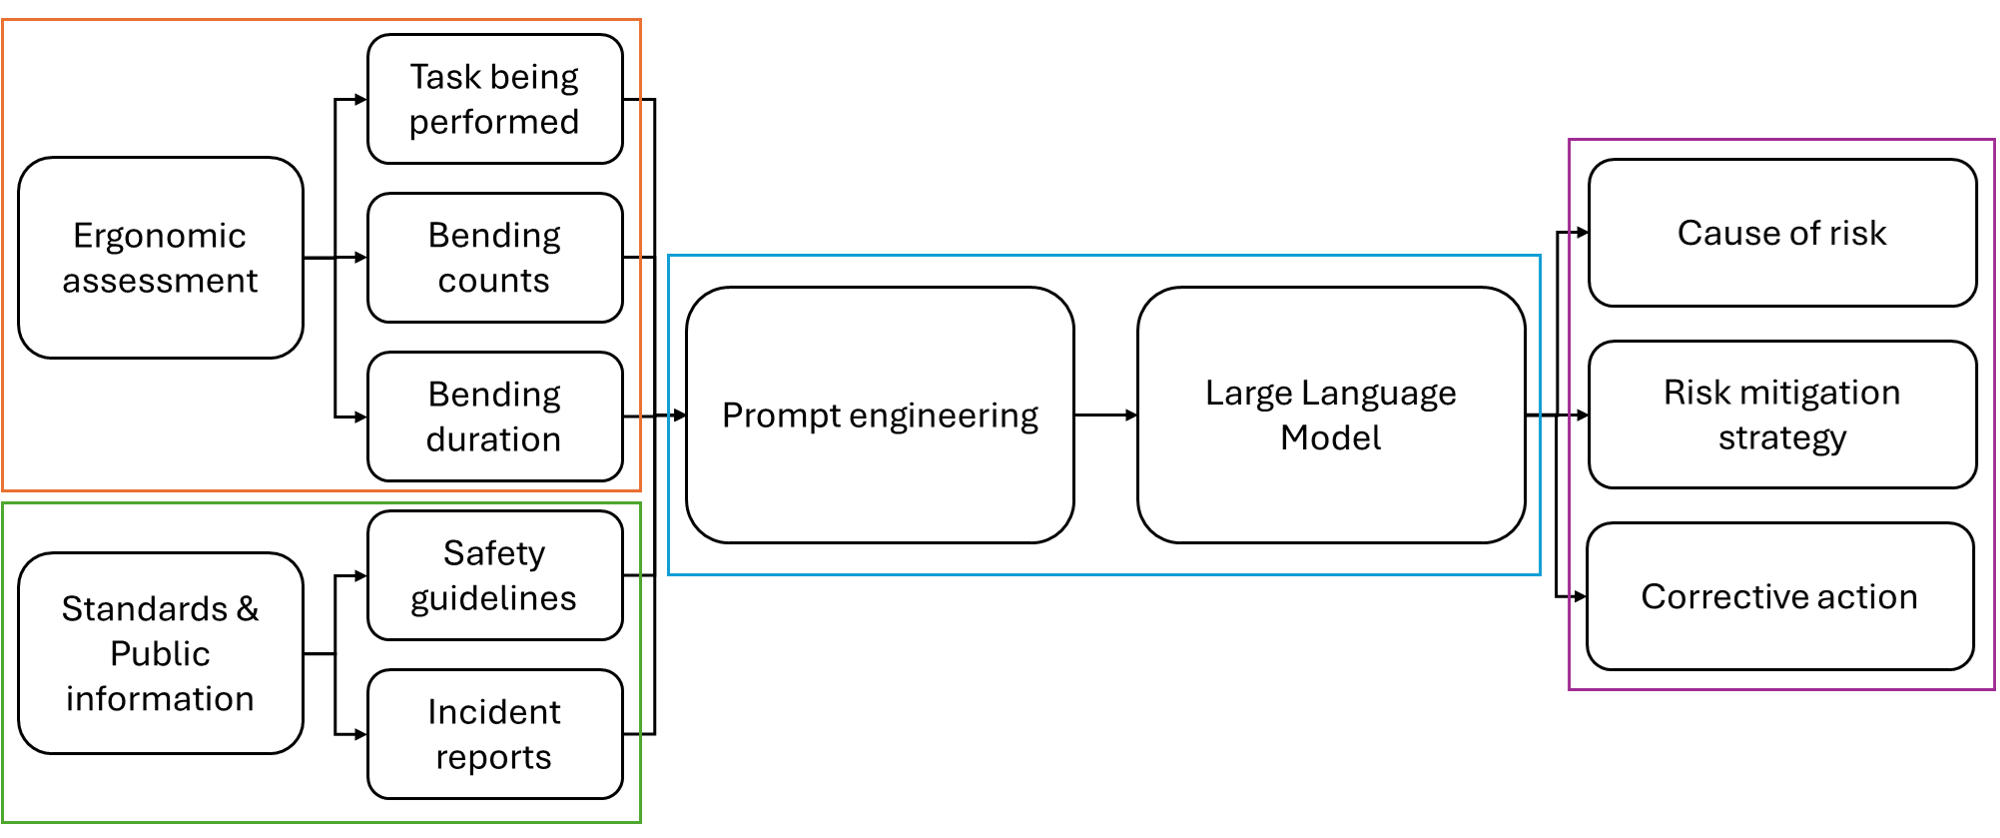
\includegraphics[width=\textwidth]{figures/LLM.png}
    \end{subfigure}
    \caption{An information flow of generating recommendations for risk mitigation strategy using LLMs} 
    \label{fig3r}
\end{figure}

% First, the information about the construction activity and risk assessment will be generated. The activity information will be produced by using vision language models such as Qwen2-VL or Molmo, which generates text description of an given image. An example prompt to generate such description is shown in \ref{table:prompts}. Then the risk assessment results will be obtained from the YOLOv8 method described earlier in this paper. Once this information is collected, a prompt will be created as shown in \ref{table:prompts}. The placeholders enclosed in angle brackets represent the content generated from models. Task descriptions are obtained from models such as Qwen2-VL vision language models. Posture related statistics such as bending counts, and bending duration of individuals, are obtained from the ergonomic risk assessment via YoLov8. These are utilized as base inputs to create a prompt for LLMs.

\begin{table}[H]
\renewcommand{\baselinestretch}{1.0}\selectfont % 只在本表内恢复正常行距
\renewcommand{\arraystretch}{0.92}              % 微调行高
\setlength{\tabcolsep}{4pt}                     % 压缩左右内边距，默认 6pt
\centering
\small
\caption{Prompts used for activity description and risk analysis}
\begin{tabular}{p{3.2cm} p{11.5cm}}
\toprule
\textbf{Prompt} & \textbf{Description} \\
\midrule
VLM Prompt & \ttfamily Please provide a detailed description of the construction worker's activity in this image, including specific actions, tools being used, and the work context if identifiable. \\[0.5em]
LLM Prompt & \ttfamily Based on the following description of a construction worker's activity from an image: <<Task description>>. <<Posture related statistics>>. \newline\newline 
Please analyze the worker’s activity and provide: 
\begin{enumerate}[nosep, leftmargin=*]
    \item <<Causes of risk>>
    \item <<Risk mitigation strategies>>
    \item <<Corrective actions>>
\end{enumerate} \\
\bottomrule
\end{tabular}
\label{table:prompts}
\end{table}

% Meanwhile, relevant standards and public information, such as safety guidelines and statistics from incident reports (e.g., \citep{albers2007simple}), are used as knowledge basis. A Retrieval-Augmented Generation (RAG) system is developed based on the knowledge basis using the latest LLM models' api such as ChatGPT, DeepSeek, and LLAMA. The above prompt will be fed into the RAG designed to retrieve answers related to cause of risk, risk mitigation strategy, and corrective action to reduce ergonomic risks, from the LLMs based on the given inputs. Through this process, this module recommends individualized ergonomic risk mitigation strategies based on the current observed activities of individuals and safety-related documentation. The recommendations generated by the LLM and RAG modules were reviewed and validated by domain experts in construction safety and ergonomics to ensure their usefulness and accuracy. In addition, the content retrieved and synthesized by the RAG system was cross-checked against authoritative safety guidelines to confirm that the outputs were reliable and grounded in correct safety knowledge.

% A structure of an appropriate prompt is organized using these five types of data related to ergonomic risks of construction workers \textbf{(Note: it would be great if we can put an example of a prompt template here)}. This allows the recommendation system to have a standardized prompt engineering process to obtain consistent and reliable outputs from the LLMs. 

% \begin{figure}[H]
% \centering
%     \begin{subfigure}[b]{0.8\textwidth}
%         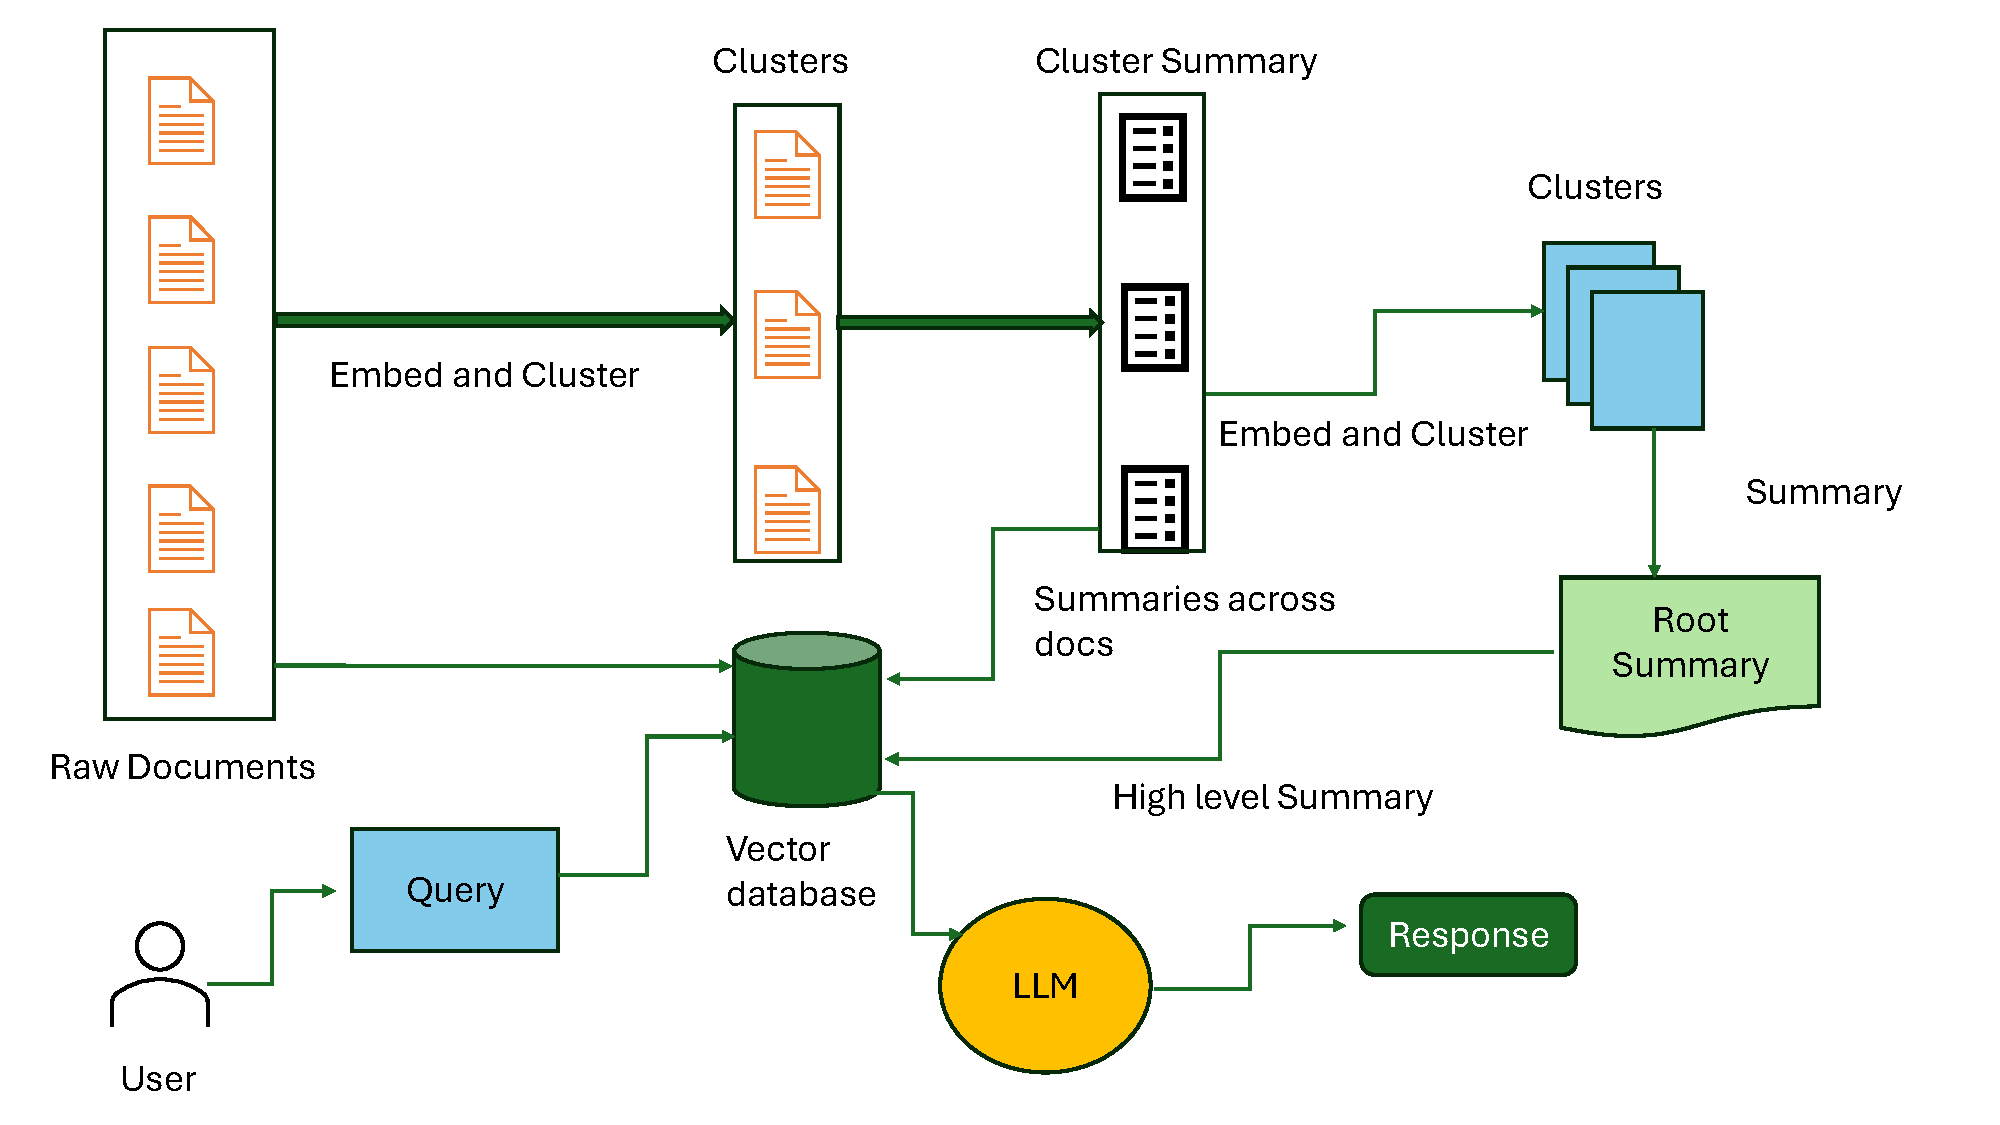
\includegraphics[width=\textwidth]{figures/figure_1.pdf}
%     \end{subfigure}
%     \caption{Framework of RAG} 
%     \label{fig:rag}
% \end{figure}

% As shown in the figure \ref{fig:rag} a typical pipeline for a Retrieval-Augmented Generation (RAG) system, where documents and questions are processed to generate a relevant answer using a language model.

% The process begins with raw documents \( D = \{d_1, d_2, \dots, d_N\} \), such as technical manuals, reports, or articles. Each document \( d_i \) is split into smaller, coherent chunks \( c_{ij} \), where \( i \) denotes the document index and \( j \) represents the chunk index. The resulting set of chunks \( C = \{c_{ij}\} \) ensures that each text chunk is manageable and semantically meaningful.

% Each text chunk \( c_{ij} \) is transformed into a high-dimensional vector embedding \( e_{ij} \) using an embedding model \( E \) (e.g., SBERT):
% \begin{equation}
% e_{ij} = E(c_{ij}), \quad e_{ij} \in \mathbb{R}^d
% \end{equation}
% Here:
% \begin{itemize}
%     \item \( E(c_{ij}) \): Embedding function mapping the chunk \( c_{ij} \) to its vector representation,
%     \item \( e_{ij} \): Embedding of the chunk,
%     \item \( d \): Dimensionality of the embedding space.
% \end{itemize}
% The embeddings for all chunks in a document \( d_i \) are grouped together as:
% \begin{equation}
% E_i = \{ e_{i1}, e_{i2}, \dots, e_{im} \}
% \end{equation}
% where \( E_i \) represents the set of embeddings for the chunks of document \( d_i \).

% These embeddings for all documents are stored in the \textbf{Knowledge Base \( V \)}, which is defined as:
% \begin{equation}
% V = \{ E_1, E_2, \dots, E_N \} 
% \end{equation}
% Here:
% \begin{itemize}
%     \item \( V \): The knowledge base containing all chunk embeddings,
% \end{itemize}

% When a user submits a query \( q \), it is embedded into a vector representation \( e_q \) using the same embedding model:
% \begin{equation}
% e_q = E(q), \quad e_q \in \mathbb{R}^d
% \label{eq:embedding}
% \end{equation}
% The query embedding \( e_q \) is compared with the document embeddings \( e_{ij} \) stored in the knowledge base \( V \) to identify the most relevant chunks. Similarity metrics, such as cosine similarity, are used to measure relevance:
% \begin{equation}
% \text{cosine\_similarity}(e_q, e_{ij}) = \frac{e_q \cdot e_{ij}}{\| e_q \| \| e_{ij} \|}
% \label{eq:cosine}
% \end{equation}
% Alternatively, Euclidean distance (L2) can be used to calculate the nearest vector:
% \begin{equation}
% \text{distance}(e_q, e_{ij}) = \| e_q - e_{ij} \|
% \end{equation}

% To handle large datasets efficiently, Approximate Nearest Neighbour (ANN) methods, such as \textbf{Scalable Nearest Neighbours (ScaNN)} or \textbf{Hierarchical Navigable Small World (HNSW)}, are employed to retrieve the top-\( k \) most relevant chunks, denoted as \( C_{\text{top-}k} \):
% \begin{equation}
% C_{\text{top-}k} = \text{ScaNN}(e_q, V) \quad \text{or} \quad C_{\text{top-}k} = \text{HNSW}(e_q, V)
% \end{equation}
% Here:
% \begin{itemize}
%     \item \( C_{\text{top-}k} \): The top-\( k \) chunks most relevant to the query embedding \( e_q \),
%     \item \( V = \{e_{ij}\} \): The knowledge base of all document embeddings,
%     \item \textbf{ScaNN (Scalable Nearest Neighbours)}: A highly efficient ANN algorithm optimized for large-scale similarity searches in high-dimensional spaces,
%     \item \textbf{HNSW (Hierarchical Navigable Small World)}: A graph-based ANN algorithm that builds a multi-layered graph structure for efficient nearest neighbor searches.
% \end{itemize}

% The retrieved chunks \( C_{\text{top-}k} \) are concatenated with the query \( q \) to form the \textbf{context}, which is the input for the language model. The context vector is represented as:
% \begin{equation}
% \text{context} = [q, c_{\text{top-}1}, c_{\text{top-}2}, \dots, c_{\text{top-}k}]
% \end{equation}

% The language model \( G \) (e.g., GPT-4 Turbo or Deepseek) processes the input context to generate a response \( r \):
% \begin{equation}
% r = G(\text{context})
% \end{equation}
% The generative model predicts the response by modeling the probability distribution over the possible sequence of tokens:
% \begin{equation}
% P(r \mid \text{context}) = \prod_{t=1}^T P(r_t \mid r_{1:t-1}, \text{context})
% \end{equation}
% Here:
% \begin{itemize}
%     \item \( r \): The generated response,
%     \item \( r_t \): The \( t \)-th token of the response,
%     \item \( P(r_t \mid r_{1:t-1}, \text{context}) \): The probability of generating token \( r_t \) given the prior tokens and the context.
% \end{itemize}

% The output \( r \) is presented to the user as the final answer, completing the RAG process.

\section{Case Study}
In this research, the system was initially tested using a regular webcam. The experiment was conducted on an Apple MacBook Pro with M3 chip. The system had 18 GB memory and ran on macOS Sequoia 15.1.1. 20 Creative Commons–licensed videos were gathered. They covered five construction activities: drywall finishing, tying rebar, kneeling creepers, hand screeding, and laying concrete block, with four videos for each activity. The videos range from 10 to 20 minutes in duration and feature an average of 2–3 participants per video, which resulted in approximately 40-60 participants in total. All recordings were captured in real construction site environments, typically filmed by a moving person. Camera heights generally ranged from approximately 1.2 to 1.7 meters above the ground that corresponded to chest or eye level of the videographer. For analysis, each video was processed into frames at a rate of one frame per second. During pose detection, every second frame was skipped to reduce computational load while preserving critical motion details. The accuracy of pose detection and activity classification was manually verified by the authors to ensure the system effectively flagged critical ergonomic risks. 

% \subsection{Pose Estimation}
% The pose estimation module of the proposed system uses YOLOv8 for the detection of key body keypoints like the head, shoulders, hips, knees, and ankles with high accuracy. During the preliminary tests, the system could capture those keypoints in real time. It also detects key points accurately by carefully validating them through a comparison with the actual poses that workers go through. 

% In this study, the coordinates of detected keypoints are represented in pixel values relative to the image frame, rather than real-world units. This choice aligns with the input format of the YOLOv8 model and enables consistent processing across varying camera setups without requiring camera calibration or depth estimation.

% \begin{figure}[H]
% \centering
%         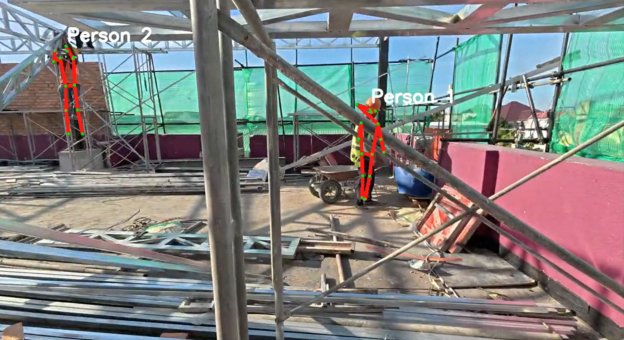
\includegraphics[width=0.4\textwidth]{figures/Pose Estimation.png}
%     \caption{Pose estimation using YOLOv8} 
%     \label{fig3}
% \end{figure}

% Figure \ref{fig3} illustrates the pose estimation result using the YOLOv8 model, applied to a scenario involving several construction workers. The video used in this figure is licensed under Creative Commons Attribution \citep{Video}. Our model successfully detects the human subjects and maps their skeletal structure with precise keypoints representing joints and limbs. These keypoints are connected to form a skeleton overlay that indicates the individual's posture and movements. This visualization demonstrates the system's ability to accurately analyze human poses in real-world environments, which is crucial for monitoring unsafe postures that could lead to injuries. For example, it can identify movements like excessive bending, twisting, or awkward lifting, which put strain on the body and increase the risk of muscle or joint injuries over time.

% However, there are still some cases where YOLOv8 is not able to identify postures and joints perfectly, such as the examples shown below.

% \begin{figure}[H]
% \centering
%     \begin{subfigure}[b]{0.45\textwidth}
%         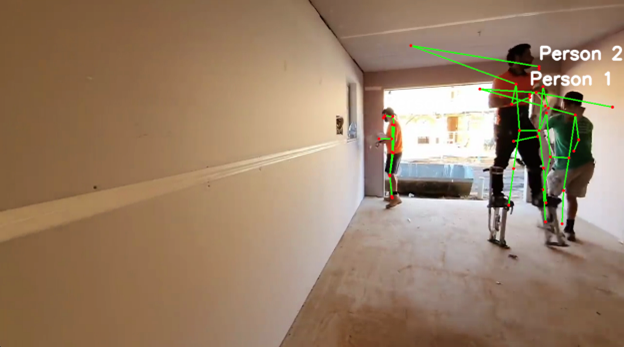
\includegraphics[width=\textwidth]{figures/Edge Case 1.png}
%         \caption{Pose detection difficulty due to multiple people and low visibility}
%         \label{fig:edge1}
%     \end{subfigure}
%     \hfill
%     \begin{subfigure}[b]{0.45\textwidth}
%         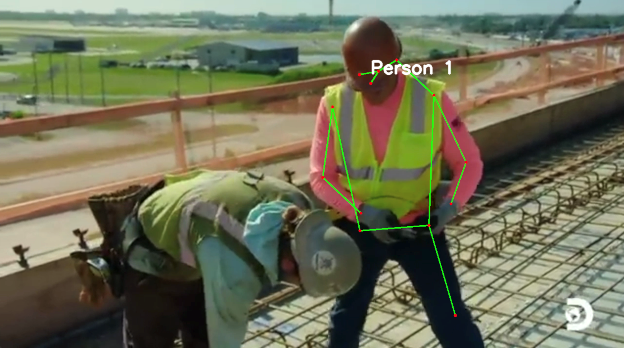
\includegraphics[width=\textwidth]{figures/Edge Case 2.png}
%         \caption{Pose detection failure due to overlapping workers}
%         \label{fig:edge2}
%     \end{subfigure}
%     \caption{Examples of pose estimation challenges}
%     \label{fig:edge_cases}
% \end{figure}

% As shown in Figure \ref{fig:edge_cases}, these are some cases where the system struggled to detect poses accurately. One example is when there are many people in the scene as shown in Figure \ref{fig:edge_cases}(a), and some are farther from the camera, making them less visible due to lower video quality. Another challenging scenario occurs when two workers overlap or stand directly in front of each other as shown in Figure \ref{fig:edge_cases}(b), causing one of them to be partially or completely unrecognized by the model. These limitations could potentially be addressed by integrating temporal information from consecutive frames, which allowes the model to infer occluded keypoints based on motion patterns. Additionally, incorporating higher-resolution video inputs or using multi-camera setups could help capture distant or partially obstructed individuals more clearly. Advanced post-processing techniques, such as keypoint tracking and interpolation, could also improve the robustness of pose estimation in challenging construction site environments.

\subsection{Landmark Smoothing}

The landmark smoothing technique is used to enhance the system's ability to generate more refined and accurate representations of workers' postures during continuous movement. Figure \ref{fig4} illustrates the impact of landmark smoothing on pose estimation using YOLOv8. Figures \ref{fig:1b}, \ref{fig:2b}, and \ref{fig:3b} show keypoint positions without smoothing  . In these unsmoothed examples, some low-confidence keypoints are returned by the pose model as the default image coordinate \((0,0)\), which is the upper-left corner of the frame. Therefore, the problem shown in Figure \ref{fig4} is not that the worker's landmark truly belongs at \((0,0)\), but that a missing or unreliable detection is encoded by the model output at that origin coordinate. If these raw coordinates are used directly, the skeleton suddenly stretches toward the upper-left corner and creates a physically implausible posture.  In contrast, Figures \ref{fig:a1}, \ref{fig:a2}, and \ref{fig:a3} present the results after applying landmark smoothing, which revealed more stable and consistent keypoint trajectories. The smoothing algorithm reduces abrupt changes by averaging each frame's landmark positions with those from previous frames by using a specified smoothing factor.  As a result, the method functions primarily as a missing-data interpolation mechanism in these examples, because it prevents a single spurious \((0,0)\) output from dominating the skeleton, while also reducing ordinary frame-to-frame jitter.  This process stabilizes the skeletal representation, which ensures a more accurate depiction of movement over time.

\begin{figure}[H]
    \centering
    % ---------------- Row 1 ----------------
    \begin{subfigure}[b]{\textwidth}
        \centering

        \begin{subfigure}[b]{0.30\textwidth}
            \centering
            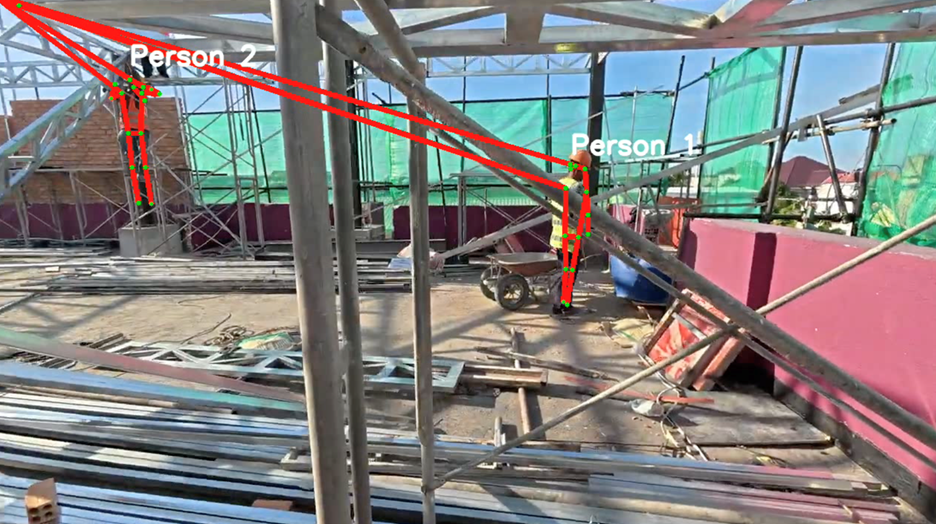
\includegraphics[width=\textwidth]{figures/Landmark Smoothing 1 - Before.png}
            \caption{Image 1 before smoothing}
            \label{fig:1b}
        \end{subfigure}\hfill
        \begin{subfigure}[b]{0.30\textwidth}
            \centering
            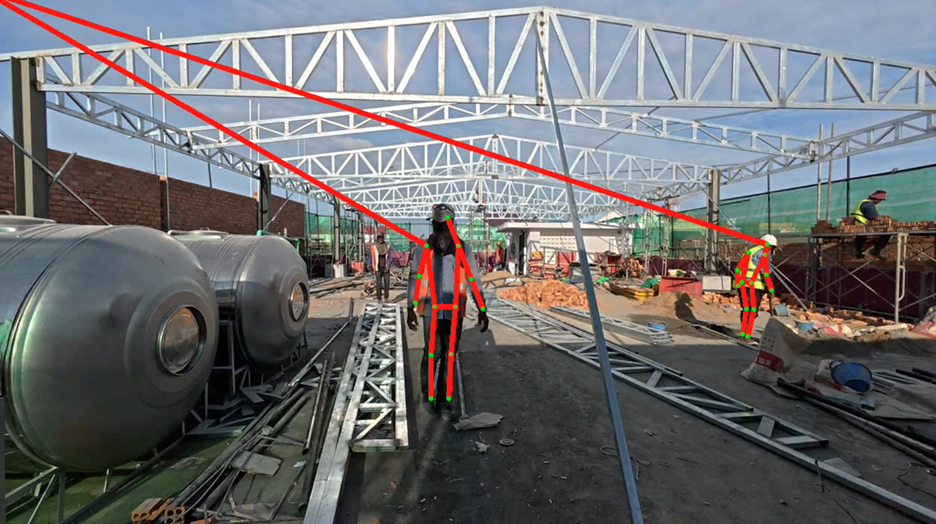
\includegraphics[width=\textwidth]{figures/Landmark Smoothing 2 - Before.png}
            \caption{Image 2  before smoothing}
            \label{fig:2b}
        \end{subfigure}\hfill
        \begin{subfigure}[b]{0.30\textwidth}
            \centering
            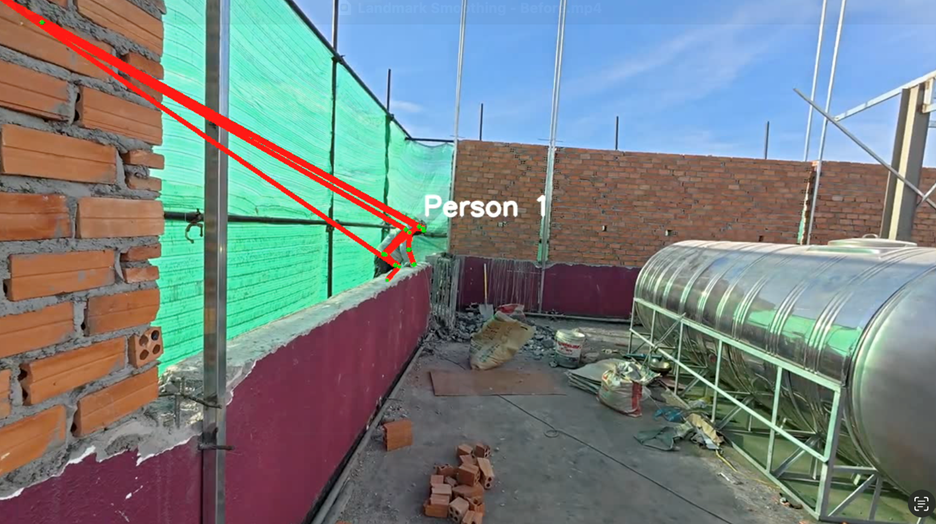
\includegraphics[width=\textwidth]{figures/Landmark Smoothing 3 - Before.png}
            \caption{Image 3  before smoothing}
            \label{fig:3b}
        \end{subfigure}
    \end{subfigure}

    % ---------------- Row 2 ----------------
    \begin{subfigure}[b]{\textwidth}
        \centering
        % \textbf{After landmark smoothing}   % row title without (e)

        \begin{subfigure}[b]{0.30\textwidth}
            \centering
            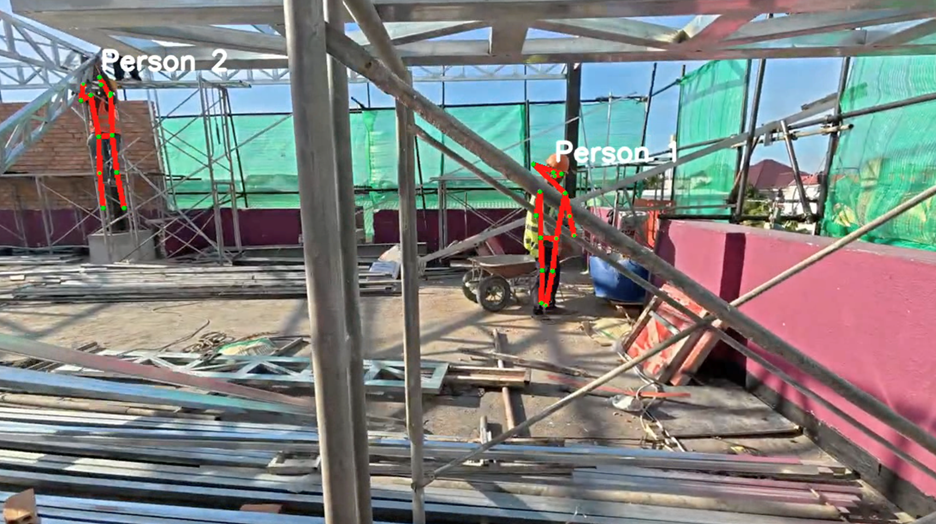
\includegraphics[width=\textwidth]{figures/Landmark Smoothing 1 - After.png}
            \caption{Image 1 after smoothing}
            \label{fig:a1}
        \end{subfigure}\hfill
        \begin{subfigure}[b]{0.30\textwidth}
            \centering
            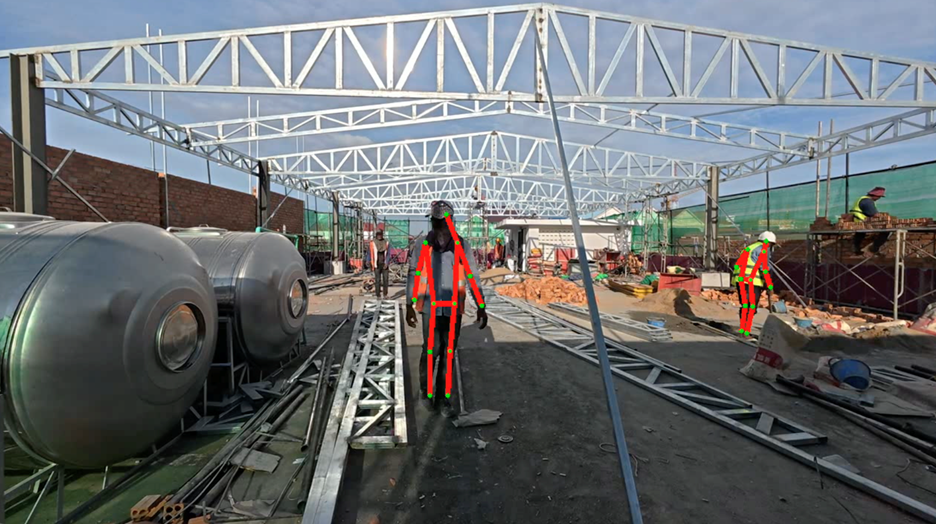
\includegraphics[width=\textwidth]{figures/Landmark Smoothing 2 - After.png}
            \caption{Image 2  after smoothing}
            \label{fig:a2}
        \end{subfigure}\hfill
        \begin{subfigure}[b]{0.30\textwidth}
            \centering
            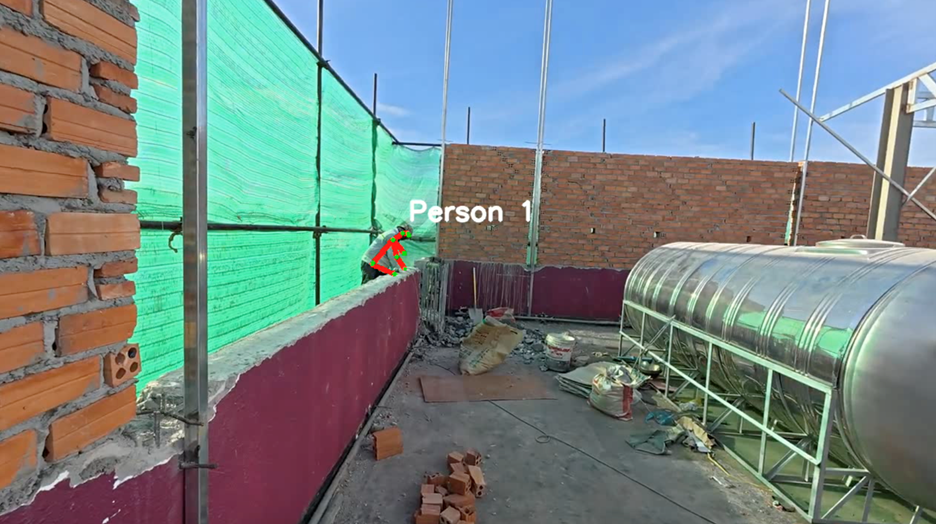
\includegraphics[width=\textwidth]{figures/Landmark Smoothing 3 - After.png}
            \caption{Image 3  after smoothing}
            \label{fig:a3}
        \end{subfigure}
    \end{subfigure}

    % ---- Overall figure caption ----
    \caption{Comparison of pose estimation with and without landmark smoothing}
    \label{fig4}
\end{figure}

 \subsection{Failure Scenarios Under Occlusion and Multi-person Overlap}

Although the qualitative examples in Figure \ref{fig5} demonstrate successful posture extraction, the model does not perform equally well in all site conditions. Figure \ref{fig:edge_cases} presents two representative failure scenarios observed in the construction videos. In Figure \ref{fig:edge1}, multiple workers appear at different depths in a narrow indoor workspace. The distant worker is only partially visible, and the workers on the right overlap spatially, which causes elongated or misplaced skeleton connections. In Figure \ref{fig:edge2}, one worker bends forward while another stands directly beside him, which creates partial body occlusion and ambiguity in separating the two individuals. In both cases, the output remains qualitatively informative, but individual joints can be misplaced and some body segments may be omitted or incorrectly connected.

These cases highlight an important limitation of the current single-camera YOLOv8-based pipeline. Performance degrades when workers overlap, when limbs are self-occluded, or when a person occupies only a small portion of the frame. Consequently, downstream measurements such as bending duration, transition counts, and REBA-based posture interpretation may become less reliable in crowded or heavily occluded scenes. Future improvements may include stronger multi-object tracking, temporal keypoint interpolation across longer windows, and multi-camera views to reduce visibility loss.

\begin{figure}[H]
\centering
    \begin{subfigure}[b]{0.47\textwidth}
        \centering
        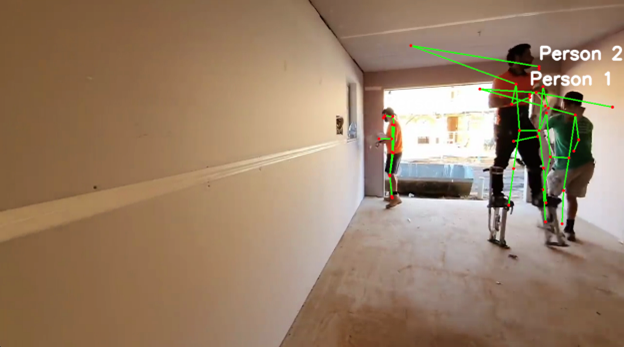
\includegraphics[width=\textwidth]{figures/Edge Case 1.png}
        \caption{Pose estimation under multi-person overlap and depth variation}
        \label{fig:edge1}
    \end{subfigure}
    \hfill
    \begin{subfigure}[b]{0.47\textwidth}
        \centering
        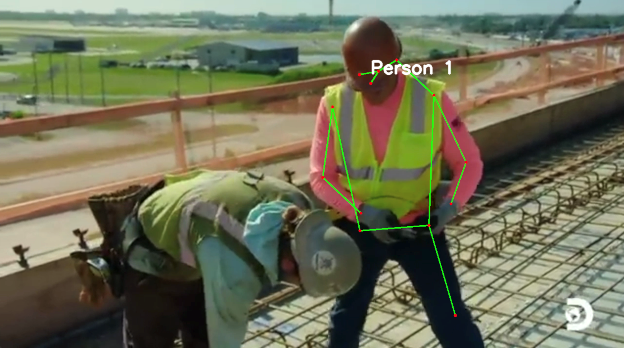
\includegraphics[width=\textwidth]{figures/Edge Case 2.png}
        \caption{Pose estimation under occlusion during a bending task}
        \label{fig:edge2}
    \end{subfigure}
    \caption{Failure scenarios for skeleton extraction in crowded and partially occluded construction scenes}
    \label{fig:edge_cases}
\end{figure}

 \subsection{Detection of Activity with Ergonomic Risks}

% In this case study, the system used smoothed keypoints to detect activities with ergonomic risks, which distinguished between standing, bending, and transition states. The tests confirmed that the system could classify continuous repetitions of bending and standing in real time. Manual verification showed that the frames were correctly classified. The following are examples of applying the proposed system to various construction activities such as drywall finishing, hand screeding, kneeling creper, laying concrete blocks, and tying rebar.

Figure \ref{fig5} shows skeletal overlays of workers performing drywall finishing tasks in three different scenarios. Drywall finishing involves the process of smoothing, taping, and sealing joints between drywall sheets after they are mounted on walls or ceilings. This work often requires individuals to bend and crouch, as they need to reach lower sections of the wall or work in confined spaces to apply compound and tape properly. Prolonged bending during drywall finishing can strain the lower back, which increases the risk of injury. Figure \ref{fig5(a)} shows a single worker labeled as   `` Person 1,  ''  who remains standing across multiple frames. The skeletal overlays display straight lines that represent the worker’s upright posture. It shows that the skeletons remain stable throughout the sequence. The figure also shows that no red lines appear in these frames, which means that no bending was detected. Figure \ref{fig5(b)} includes two workers labeled as   `` Person 1  '' and `` Person 2.  ''  Each worker seem to perform different activities over time.   `` Person 1  ''  moves between normal and risky postures.   `` Person 2  ''  remains in normal posture without changes. Figure \ref{fig5(c)} illustrates the activities of   `` Person 2  ''  across a sequence of frames. The worker alternates between standing and bending. 

% \subsubsection{Drywall Finishing}
\begin{figure}[H]
    \centering
    % Row 1
    \begin{subfigure}[b]{0.45\textwidth}
        \centering
        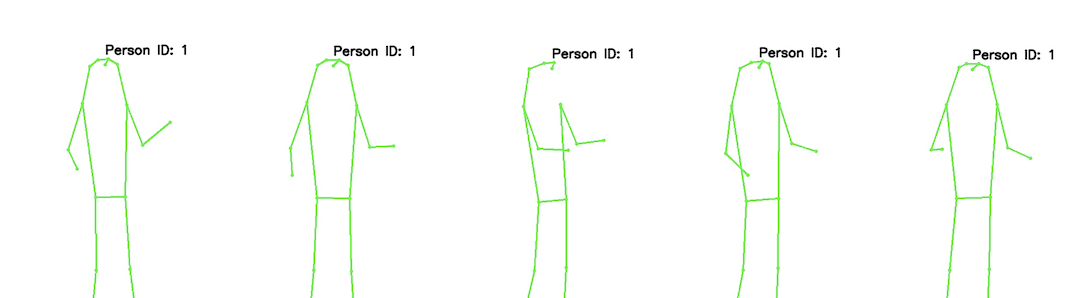
\includegraphics[width=\textwidth]{figures/Drywall Finishing Test 1.png}
        \caption{Scenario 1}
        \label{fig5(a)}
    \end{subfigure}
    % \vspace{-0.5\baselineskip}
    \hfill
    % Row 2
    \begin{subfigure}[b]{0.45\textwidth}
        \centering
        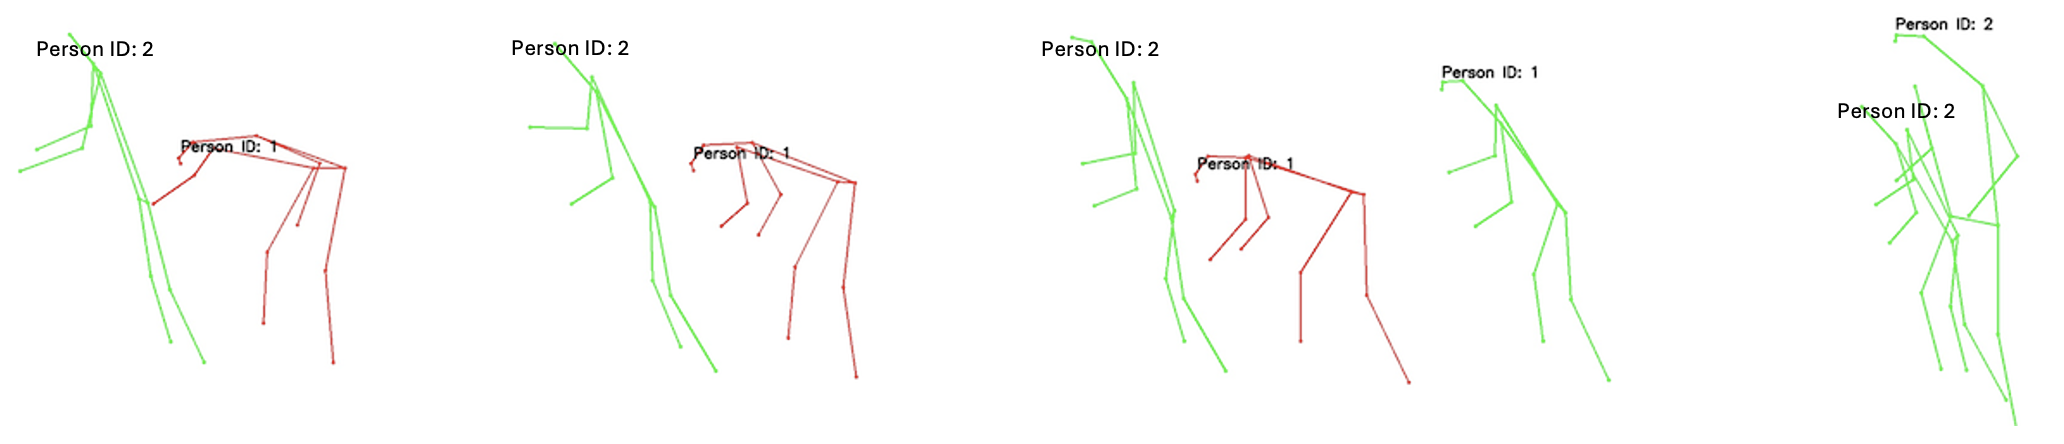
\includegraphics[width=\textwidth]{figures/Drywall Finishing Test 2.png}
        \caption{Scenario 2}
        \label{fig5(b)}
    \end{subfigure}
    % \vspace{-0.5\baselineskip} % Space between rows
    % \hfill
    % Row 3
    \begin{subfigure}[b]{0.5\textwidth}
        \centering
        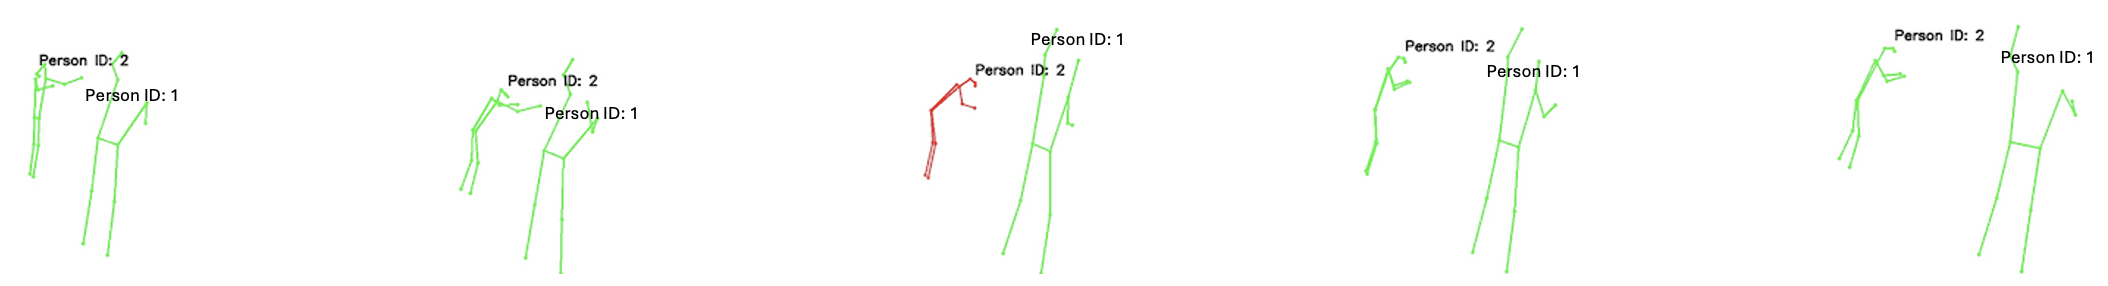
\includegraphics[width=\textwidth]{figures/Drywall Finishing Test 3.png}
        \caption{Scenario 3}
        \label{fig5(c)}
    \end{subfigure}

    \caption{Skeleton Representation of Workers Performing Drywall Finishing (Red: Ergonomic Risk Activity)
}
    \label{fig5}
\end{figure}

% \subsubsection{Hand Screeding}

Figure \ref{fig6} depicts skeletal overlays of workers' performing hand screeding. Hand screeding is a labor intensive process used in construction to level and smooth concrete surfaces. This activity uses a flat board or screed to spread the concrete evenly across the surface. Workers often need to bend and stoop while performing this task to ensure an even and level finish. During hand screeding, repetitive bending and awkward postures can place significant strain on the back, especially during prolonged tasks. Figure \ref{fig6(a)} shows multiple workers labeled as   `` Person 1  '' to `` Person 4.  ''  The majority are in normal posture, represented by green skeletons, while   `` Person 1  ''  transitions into bending, shown with red skeletons. Figure \ref{fig6(b)} focuses on two workers,   `` Person 1  '' and `` Person 2,  ''  actively alternating between standing and bending.   `` Person 1  ''  shows a mix of standing and bending postures, visualized through alternating green and red skeletons.   `` Person 2  ''  primarily shows ergonomically risky postures, represented by red skeletons. Figure \ref{fig6(c)} includes a group of workers labeled from   `` Person 1  '' to `` Person 6.  ''  The skeletal overlays illustrate a variety of activities, with some individuals standing consistently and others bending intermittently.   `` Person 3  '' and `` Person 5  ''  exhibit frequent bending motions, indicated by red skeletons, while   `` Person 4  '' and `` Person 6  ''  remain standing throughout the sequence. 

\begin{figure}[H]
    \centering
    % Row 1
    \begin{subfigure}[b]{0.7\textwidth}
        \centering
        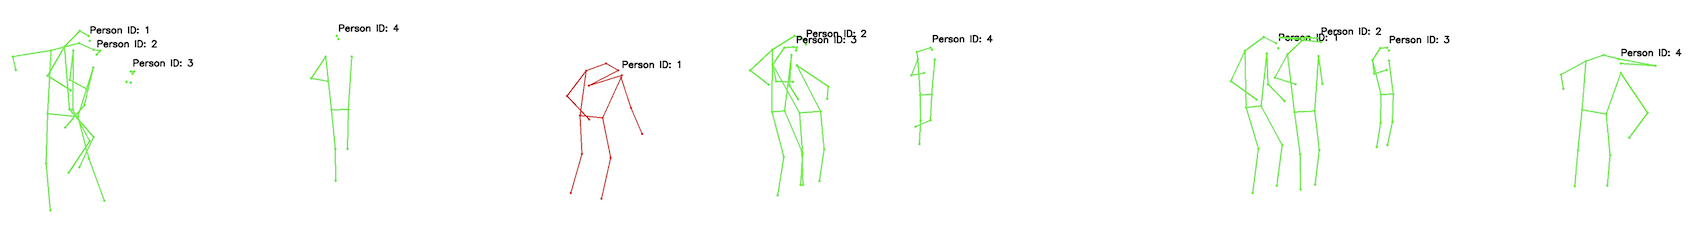
\includegraphics[width=\textwidth]{figures/Hand Screeding Test 1.png}
        \caption{Scenario 1}
        \label{fig6(a)}
    \end{subfigure}

    % \vspace{-0.5\baselineskip} % Space between rows

    % Row 2
    \begin{subfigure}[b]{0.7\textwidth}
        \centering
        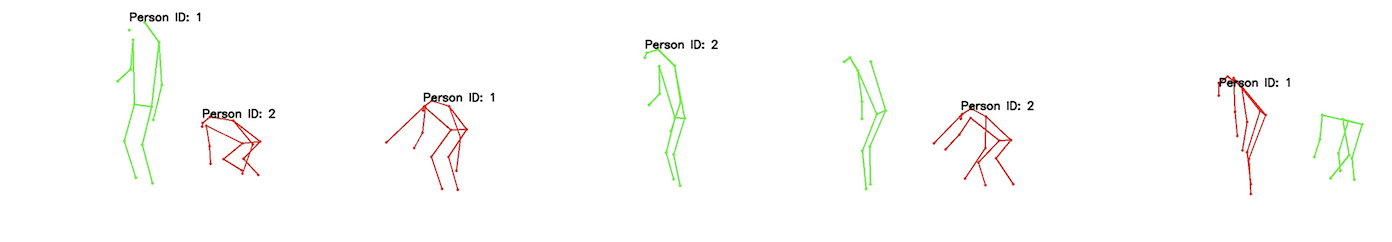
\includegraphics[width=\textwidth]{figures/Hand Screeding Test 2.png}
        \caption{Scenario 2}
        \label{fig6(b)}
    \end{subfigure}
    % \vspace{-0.5\baselineskip} % Space between rows

    % Row 3
    \begin{subfigure}[b]{0.7\textwidth}
        \centering
        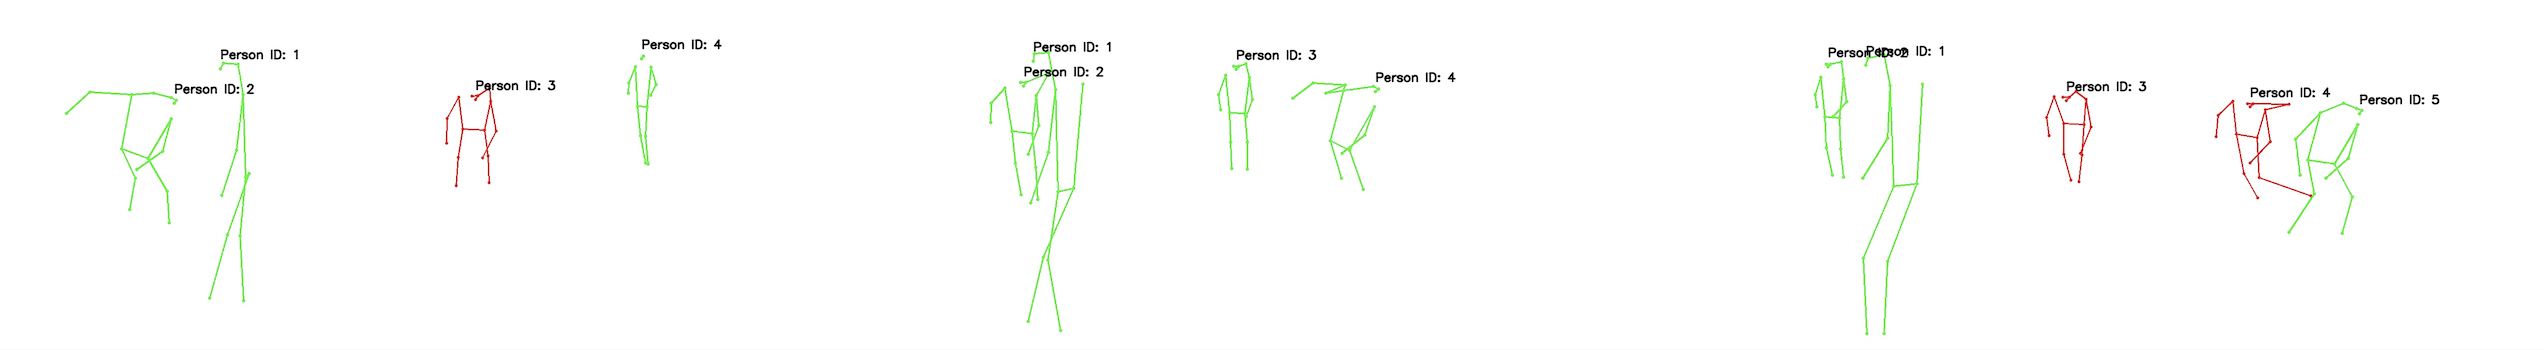
\includegraphics[width=\textwidth]{figures/Hand Screeding Test 3.png}
        \caption{Scenario 3}
        \label{fig6(c)}
    \end{subfigure}
    \caption{Skeleton representation of workers performing hand screeding over consecutive frames at 1-second intervals}
    \label{fig6}
\end{figure}

% \subsubsection{Kneeling Creeper}

Figure \ref{fig7} depicts skeletal overlays of workers' performing kneeling finishing. Kneeling finishing are used in construction and other manual tasks where workers need to spend extended periods kneeling on hard surfaces, such as during tasks like tiling, plumbing, or electrical work. Kneeling for long durations can lead to discomfort, joint pain, and strain on the knees and lower back. This repetitive pressure can be physically taxing, especially in environments where the worker must stay in a kneeling position for long periods. Figure \ref{fig7(a)} shows two workers labeled as   `` Person 1  '' and `` Person 2.  '' `` Person 1  ''  is predominantly engaged in bending postures, represented by red skeletons, while   `` Person 2  ''  alternates between standing and bending. Figure \ref{fig7(b)} focuses on   `` Person 1,  ''  demonstrating repeated transitions between bending and standing postures. The red skeletons depict periods of kneeling, while the green skeletons represent standing intervals. Figure \ref{fig7(c)} includes a detailed sequence for   `` Person 1,  ''  which shows transitions from bending to standing over several frames. 

\begin{figure}[H]
    \centering

    % Row 1
    \begin{subfigure}[b]{0.9\textwidth}
        \centering
        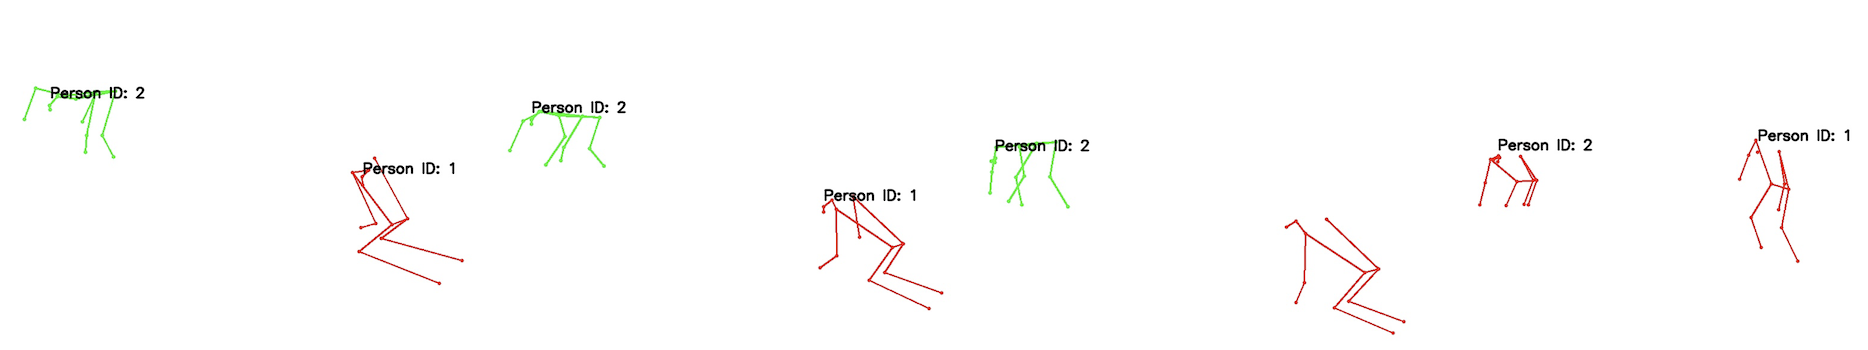
\includegraphics[width=\textwidth]{figures/Kneeling Creeper Test 1.png}
        \caption{Scenario 1}
        \label{fig7(a)}
    \end{subfigure}

    % \vspace{-0.5\baselineskip} % Space between rows

    % Row 2
    \begin{subfigure}[b]{0.6\textwidth}
        \centering
        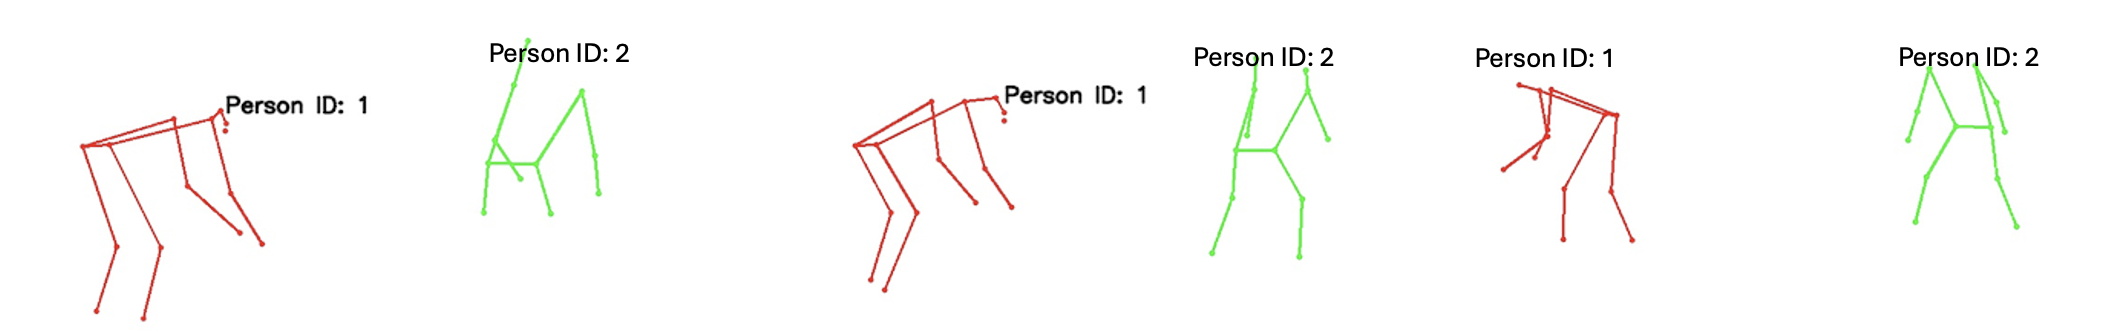
\includegraphics[width=\textwidth]{figures/Kneeling Creeper Test 2.png}
        \caption{Scenario 2}
        \label{fig7(b)}
    \end{subfigure}
    \hfill
    % Row 3
    \begin{subfigure}[b]{0.2\textwidth}
        \centering
        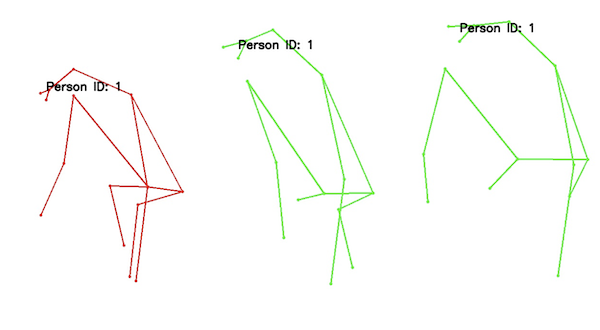
\includegraphics[width=\textwidth]{figures/Kneeling Creeper Test 3.png}
        \caption{Scenario 3}
        \label{fig7(c)}
    \end{subfigure}    

    \caption{Skeleton representation of workers performing kneeling creepers over consecutive frames at 1-second intervals}
    \label{fig7}
\end{figure}

% \subsubsection{Laying Concrete Block}

Figure \ref{fig8} depicts skeletal overlays of workers' laying concrete blocks. Laying concrete blocks is a physically demanding task that requires workers to lift, position, and align heavy blocks to create walls or other structures. This often involves bending, lifting, and repetitive motions, which can cause strain on the back, shoulders, and arms, especially when working with traditional, heavy concrete blocks. Constantly lifting and manipulating these blocks over extended periods can lead to fatigue and increase the risk of musculoskeletal injuries. Figure \ref{fig8(a)} shows   `` Person 1  ''  engaged in bending activities across multiple frames. Figure \ref{fig8(b)} includes two workers,   `` Person 1  '' and `` Person 2.  '' `` Person 1  ''  alternates between standing and bending postures, shown by the mix of green and red skeletons, while   `` Person 2  ''  remains consistently standing. Figure \ref{fig8(c)} focuses on   `` Person 1  ''  maintaining a standing posture across several frames. 

\begin{figure}[H]
    \centering
    % Row 1
    \begin{subfigure}[b]{0.4\textwidth}
        \centering
        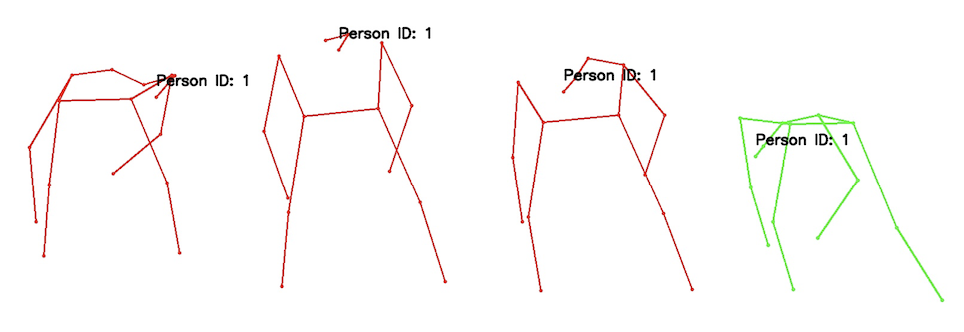
\includegraphics[width=\textwidth]{figures/Laying Concrete Block Test 1.png}
        \caption{Scenario 1}
        \label{fig8(a)}
    \end{subfigure}
    \hfill
    % Row 3
    \begin{subfigure}[b]{0.4\textwidth}
        \centering
        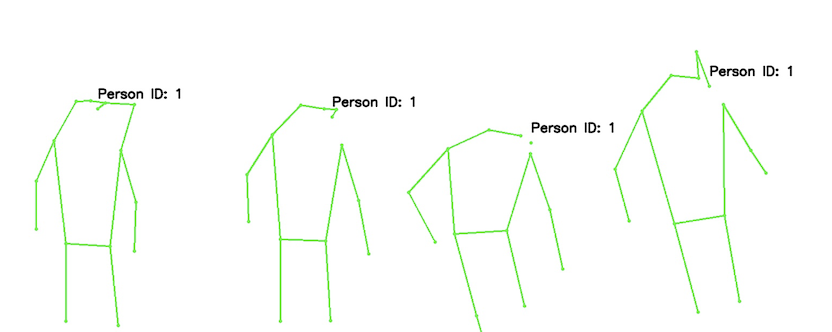
\includegraphics[width=\textwidth]{figures/Laying Concrete Block Test 3.png}
        \caption{Scenario 3}
        \label{fig8(c)}
    \end{subfigure}    
    % Row 2
    \begin{subfigure}[b]{0.9\textwidth}
        \centering
        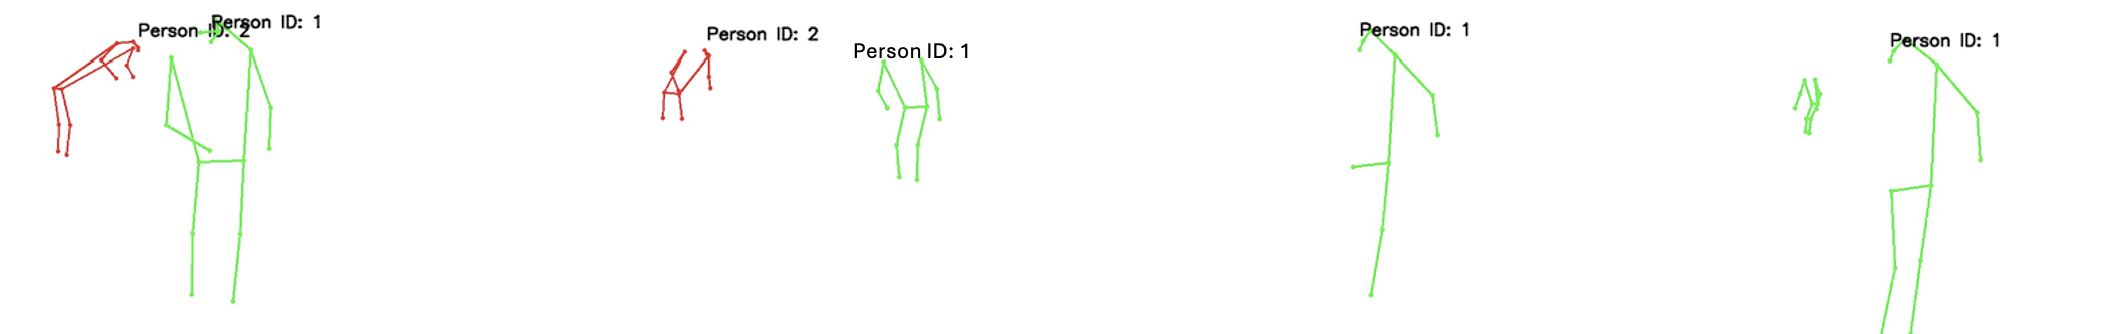
\includegraphics[width=\textwidth]{figures/Laying Concrete Block Test 2.png}
        \caption{Scenario 2}
        \label{fig8(b)}
    \end{subfigure}
    % \vspace{-0.5\baselineskip} % Space between rows

    \caption{Skeleton representation of workers laying concrete blocks over consecutive frames at 1-second intervals}
    \label{fig8}
\end{figure}

% \subsubsection{Tying Rebar}

Figure \ref{fig9} depicts skeletal overlays of workers' tying rebar.  Tying rebar requires workers to bend, twist, and secure metal rebar with wire ties. This task involves repetitive hand movements and awkward postures, often requiring workers to bend down or crouch for long periods. This can lead to strain on the back, hands, and wrists. The repetitive nature of tying rebar also increases the risk of hand injuries or discomfort from prolonged gripping. Figure \ref{fig9(a)} shows two workers,   `` Person 1  '' and `` Person 2,  ''  predominantly engaged in bending activities. The red skeletons represent bending postures consistently, with multiple frames showing   `` Person 1  ''  bending, while   `` Person 2  ''  is seen bending in the middle of the sequence. Figure \ref{fig9(b)} features   `` Person 1  '' and `` Person 2,  ''  both transitioning between standing and bending postures.   `` Person 1  ''  shows a more upright posture in most frames, while   `` Person 2  ''  demonstrates intermittent bending. Figure \ref{fig9(c)} focuses on the activity of   `` Person 2  ''  and demonstrates transitions from standing to bending and back to standing. 

\begin{figure}[H]
    \centering
    % Row 1
    \begin{subfigure}[b]{0.9\textwidth}
        \centering
        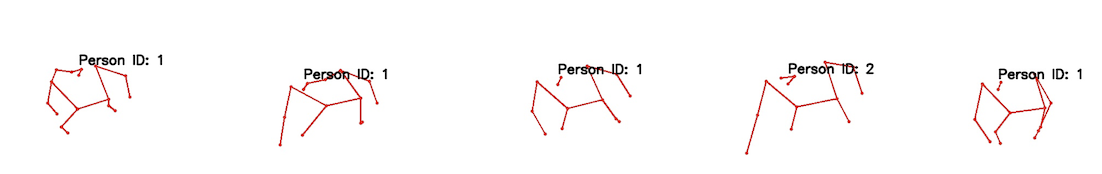
\includegraphics[width=\textwidth]{figures/Tying Rebar Test 1.png}
        \caption{Scenario 1}
        \label{fig9(a)}
    \end{subfigure}
    % Row 2
    \begin{subfigure}[b]{0.7\textwidth}
        \centering
        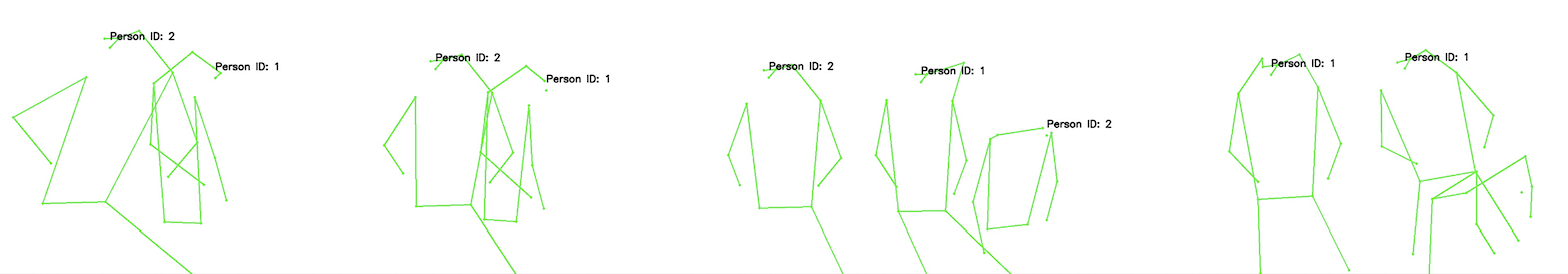
\includegraphics[width=\textwidth]{figures/Tying Rebar Test 2.png}
        \caption{Scenario 2}
        \label{fig9(b)}
    \end{subfigure}
    % Row 3
    \begin{subfigure}[b]{0.9\textwidth}
        \centering
        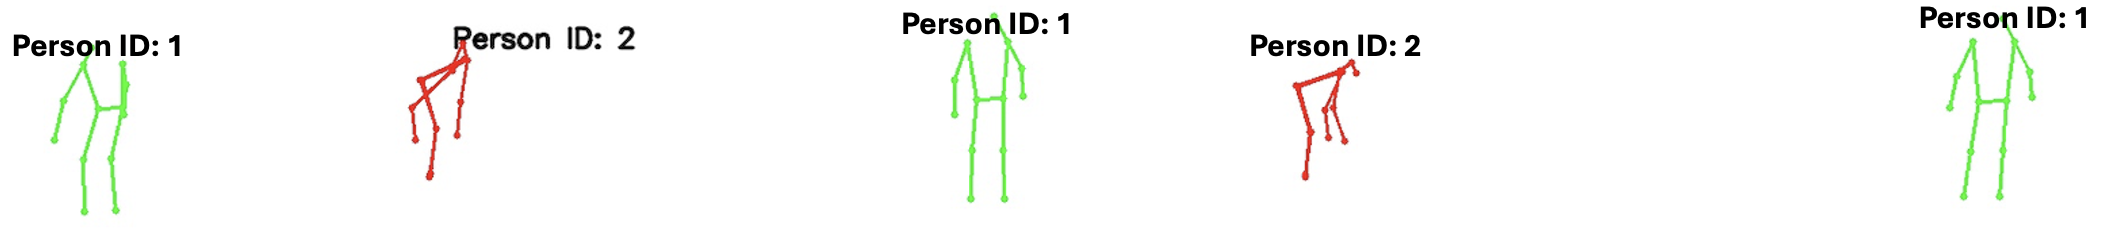
\includegraphics[width=\textwidth]{figures/Tying Rebar Test 3.png}
        \caption{Scenario 3}
        \label{fig9(c)}
    \end{subfigure}
    \caption{Skeleton representation of workers tying rebar over consecutive frames at 1-second intervals}
    \label{fig9}
\end{figure}

\subsection{Activity Duration and Count}

The developed system is also able to track the duration and count of normal and risky postures, as well as how often workers switch between them. Figure \ref{fig10} illustrates an example to track and visualize activity duration and bending count for a construction worker labeled as   `` Person 1.  ''  The worker’s posture is classified as   ``Bending''  (red) and   ``Standing''  (green) based on the alignment of key body landmarks such as the nose, shoulders, hips, and ankles. The bending duration is shown in red, with times of 5 seconds, 3 seconds, and 2 seconds recorded for three separate intervals. Similarly, the standing duration is shown in green, with times of 1 second and 4 seconds between bending intervals. The bending count is updated each time the worker transitions from standing to bending, as indicated by the arrows in the image. In this example, the bending count increases by 1 twice during the session, resulting in a total bending count of 2. 

\begin{figure}[H]
\centering
\begin{subfigure}[b]{0.7\textwidth}
    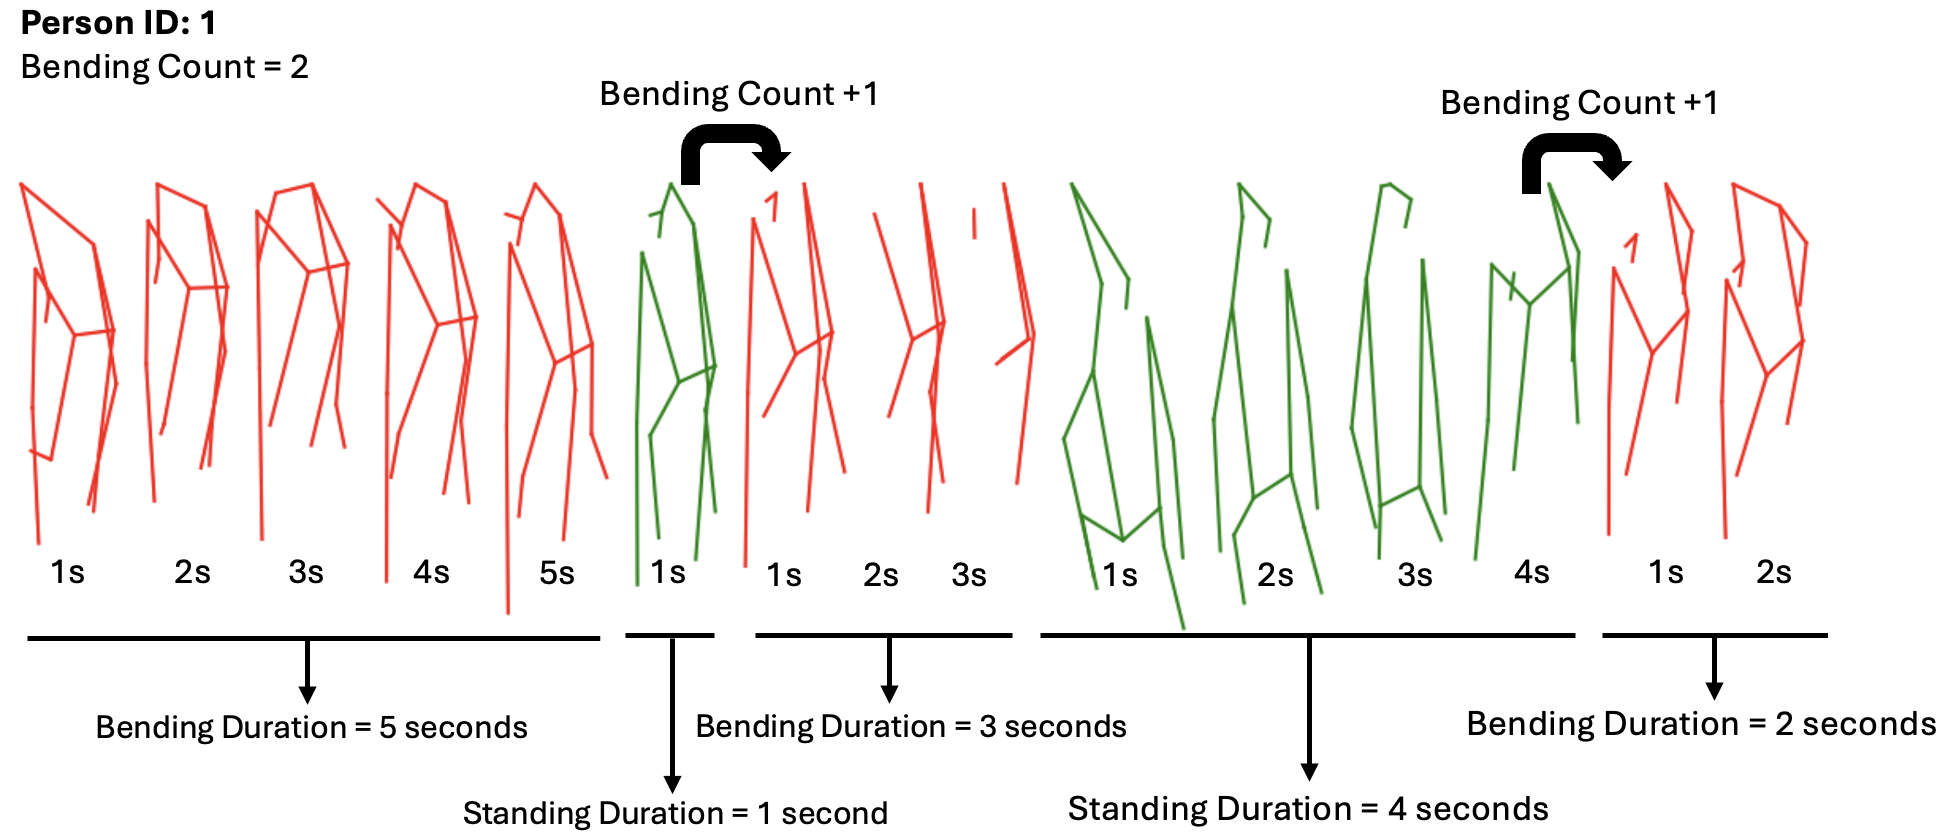
\includegraphics[width=\textwidth]{figures/Activity Duration and Bending Count.png}
\end{subfigure}
\caption{Displaying Activity Duration and Bending Count}
\label{fig10}
\end{figure}

\subsection{Comparison of Model and Manual Evaluation}
We conducted a comparison of model generated and manually recorded activity data to evaluate the system's accuracy in detecting ergonomic risk factors. To establish a ground truth for comparison, human observers manually reviewed recorded videos of workers performing these scenarios. They identified postural changes and recorded their duration and count. By comparing the model's detections with these manually recorded values, we calculated the error rate. The error rate quantifies the percentage difference between the two methods. The error rate was determined using the following formula:

\begin{equation}  
E_{\mathrm{final}} = \frac{100}{3}
\left(
   \frac{\lvert M_{\mathrm{np}} - G_{\mathrm{np}} \rvert}{G_{\mathrm{np}}}
 + \frac{\lvert M_{\mathrm{er}} - G_{\mathrm{er}} \rvert}{G_{\mathrm{er}}}
 + \frac{\lvert M_{\mathrm{freq}} - G_{\mathrm{freq}} \rvert}{G_{\mathrm{freq}}}
\right)
\end{equation}

\noindent where,\\
$E_{\mathrm{final}}$  = Final average error percentage;\\
$M_{\mathrm{np}},\, G_{\mathrm{np}}$  = Model and ground truth values for normal posture duration;\\
$M_{\mathrm{er}},\, G_{\mathrm{er}}$ = Model and ground truth values for ergonomically risky duration;\\
$M_{\mathrm{freq}},\, G_{\mathrm{freq}} $ = Model and ground truth values for count of risky activity.

Table \ref{table1} shows a detailed comparison of manual and model evaluations for different construction related tasks. Each task is broken down into multiple test scenarios. The table reports three main metrics for each scenario: duration of normal posture in seconds, duration of ergonomically risky posture in seconds, and the count of risky activities. The final column presents the error rate, which represents the difference between the model's results and manual observations. Many scenarios show low error rates. This indicates that the model tracks posture durations and frequencies accurately. For instance,   `` Hand Screeding Scenario 3  '' and `` Kneeling Creeper Scenario 2  ''  both achieve a 0 percent error rate. In these tests, the model’s metrics match the manual measurements perfectly. Tasks like   `` Hand Screeding Scenario 1  ''  also demonstrate a fairly low error rate of 2.45 percent. Some scenarios reveal moderate to higher discrepancies.   `` Tying Rebar Scenario 1  ''  shows an error rate of 5.36 percent. This higher value suggests that the model may struggle with frequent or subtle changes in posture. Rapid transitions between normal and risky positions can create more counting errors. Minor variations in how workers perform each task may further complicate detection. Sensor calibration or environmental factors like lighting can also affect the model's accuracy. Activities like   `` Hand Screeding Scenario 2  '' and `` Kneeling Creeper Scenario 3  ''  display error rates of 5.13 percent and 6.06 percent, respectively. These rates highlight potential challenges in distinguishing borderline postures or counting movements that happen quickly. Consistent repetition or variations in a task can lead to partial misclassifications. As a result, the model's readings may differ from the manual ground truth. In contrast,   `` Laying Concrete Block Scenario 1  '' and `` Tying Rebar Scenario 2  ''  each show an error rate of 0 percent. These scenarios point to conditions where the model excels at identifying posture transitions. Fewer rapid movements or clearer distinctions between normal and risky postures can reduce miscalculations. Stable lighting or simpler task patterns may also support accurate posture detection. 

% \begin{table}[H]
% \centering
% \small
% \caption{Comparison of Model and Manual Evaluations}
% \renewcommand{\arraystretch}{1}  % Adjust row height
% \setlength{\tabcolsep}{6pt}       % Adjust column spacing
% \begin{tabular}{lccc ccc c}
% \toprule
% \multirow{2}{*}{\textbf{Activity}} 
% & \multicolumn{3}{c}{\textbf{Model Evaluation}} 
% & \multicolumn{3}{c}{\textbf{Manual Evaluation}} 
% & \multirow{2}{*}{\textbf{Error Rate}} \\
% \cmidrule(lr){2-4}\cmidrule(lr){5-7}
% & \textbf{\scriptsize Standing} & \textbf{\scriptsize Bending} & \textbf{\scriptsize Bending} 
% & \textbf{\scriptsize Standing} & \textbf{\scriptsize Bending} & \textbf{\scriptsize Bending} 
% &  \\
% & \textbf{\scriptsize Duration} & \textbf{\scriptsize Duration} & \textbf{\scriptsize Count} 
% & \textbf{\scriptsize Duration} & \textbf{\scriptsize Duration} & \textbf{\scriptsize Count} 
% &  \\
% \midrule
% Hand Screeding Scenario 1 & 105 & 12 & 92 & 102 & 12 & 90 & 2.45 \\
% Hand Screeding Scenario 2 & 35 & 22 & 107 & 35 & 21 & 100 & 5.13 \\
% Hand Screeding Scenario 3 & 53 & 7 & 47 & 53 & 7 & 47 & 0.00 \\
% Drywall Finishing Scenario 1 & 20 & 10 & 3 & 20 & 9 & 3 & 3.13 \\
% Drywall Finishing Scenario 2 & 61 & 7 & 33 & 59 & 7 & 33 & 2.02 \\
% Drywall Finishing Scenario 3 & 45 & 3 & 15 & 45 & 3 & 15 & 0.00 \\
% Laying Concrete Block Scenario 1 & 31 & 0 & 0 & 31 & 0 & 0 & 0.00 \\
% Laying Concrete Block Scenario 2 & 17 & 5 & 19 & 16 & 5 & 19 & 2.50 \\
% Laying Concrete Block Scenario 3 & 60 & 13 & 78 & 55 & 13 & 78 & 4.79 \\
% Kneeling Creeper Scenario 1 & 65 & 9 & 25 & 65 & 9 & 25 & 0.00 \\
% Kneeling Creeper Scenario 2 & 0 & 5 & 0 & 0 & 5 & 0 & 0.00 \\
% Kneeling Creeper Scenario 3 & 11 & 6 & 14 & 11 & 8 & 14 & 6.06 \\
% Tying Rebar Scenario 1 & 15 & 12 & 32 & 14 & 12 & 30 & 5.36 \\
% Tying Rebar Scenario 2 & 2 & 4 & 2 & 2 & 4 & 2 & 0.00 \\
% Tying Rebar Scenario 3 & 36 & 9 & 31 & 35 & 9 & 31 & 1.33 \\
% \bottomrule
% \end{tabular}

% \label{table1}
% \end{table}

\begin{table}[H]
\centering
\scriptsize
\caption{Comparison of     model   and     manual bending estimates  }
\setlength{\tabcolsep}{4pt} % Compact column spacing
\renewcommand{\arraystretch}{0.95} % Compact row height
    \begin{adjustbox}{max width=\textwidth}
\begin{tabular}{llccccc}
  \toprule
    \textbf{Task}   &   \DIFaddFL{ %DIF > DIFAUXCMD
 \textbf%DIF > DIFAUXCMD
 } 
 %DIF > DIFAUXCMD
 \DIFdelendFL  \textbf{Case}  & \DIFaddFL{ %DIF > DIFAUXCMD
 \textbf%DIF > DIFAUXCMD
 } 
 \DIFdelendFL  \textbf{Model Bend Dur.}   &     \textbf{  Manual Bend Dur. }    & \textbf{    Model   Bend     Cnt  .} & \textbf{    Manual   Bend Cnt.} &   %DIF > DIFDELCMD < \scriptsize %%%
    %DIF > DIFAUXCMD
\textbf{ %DIF > DIFDELCMD < \scriptsize %%%
  }  %DIF > DIFAUXCMD
\textbf{ %DIF > DIFDELCMD < \scriptsize %%%
  } 
 %DIF > DIFAUXCMD
 \DIFdelendFL  \textbf{Error (\%)}   \\
\midrule
    \multirow{3}{*}{Hand Screeding} &   1 &     12   & 12 & 92 &     90 & 2.45 \\
     &   2 &     22 &     21 &   107 &   100 & 5.13 \\
     &   3 &     7   & 7 & 47 &     47 & 0.00 \\
    \multirow{3}{*}{Drywall Finish} &   1 &     10 &     9 & 3 &   3 &   3.13 \\
     &   2 &     7   & 7 & 33 &     33 & 2.02 \\
     &   3 &     3   & 3 & 15 &     15 & 0.00 \\
    \multirow{3}{*}{Concrete Block} &   1 &     0 & 0 &     0 & 0 & 0.00 \\
     &   2 &     5   & 5 & 19 &     19 & 2.50 \\
     &   3 &     13   & 13 & 78 &     78 & 4.79 \\
    \multirow{3}{*}{Kneeling Creeper} &   1 &     9   & 9 & 25 &     25 & 0.00 \\
     &   2 &     5   & 5 & 0 & 0 &     0.00 \\
     &   3 &     6 &     8 & 14 &   14 &   6.06 \\
    \multirow{3}{*}{Tying Rebar} &   1 &     12   & 12 & 32 &     30 & 5.36 \\
     & 2 & 4 &     4   & 2 &     2 & 0.00 \\
     &   3 &     9   & 9 & 31 &     31 & 1.33 \\
\bottomrule
\end{tabular}
  \end{adjustbox}
  \label{table1}
\end{table}

  \subsection{Full-body REBA Scoring Examples}

To demonstrate that the revised system computes full-body REBA rather than only trunk-based scoring, five representative examples are shown in Figures \ref{fig:reba_examples_a} and \ref{fig:reba_examples_b}. In each case, the system detects body keypoints, computes segment angles, converts them into segment-level REBA scores, combines them through Table A, Table B, and Table C, adds the load/force score, and outputs the final REBA score and associated risk level. The load/force term in these examples is obtained through the VLM-assisted approximate estimation workflow described in Section 3.4.

Cases 1, 4, and 5 produce high or very high REBA scores because they combine pronounced trunk flexion with elevated arm posture and unstable lower-limb support. Cases 2 and 3 produce medium-risk scores, reflecting less severe whole-body loading despite visible non-neutral posture. These examples illustrate that the revised pipeline now evaluates neck, trunk, upper arm, lower arm, wrist, legs, and load/force together, rather than reporting only a trunk-derived index.

\begin{table}[H]
\centering
\scriptsize
\caption{Summary of five full-body REBA scoring examples}
\setlength{\tabcolsep}{5pt}
\renewcommand{\arraystretch}{0.95}
\begin{tabular}{lccccc}
\toprule
\textbf{Case} & \textbf{Score A} & \textbf{Score B} & \textbf{Load} & \textbf{Final REBA} & \textbf{Risk Level} \\
\midrule
Case 1 & 7 & 5 & 2 & 9 & High \\
Case 2 & 5 & 4 & 2 & 5 & Medium \\
Case 3 & 4 & 4 & 2 & 4 & Medium \\
Case 4 & 10 & 4 & 2 & 11 & Very High \\
Case 5 & 8 & 4 & 2 & 9 & High \\
\bottomrule
\end{tabular}
\label{table:reba_examples}
\end{table}

\begin{figure}[H]
\centering
    \begin{subfigure}[b]{0.48\textwidth}
        \centering
        \includegraphics[width=\textwidth]{figures/reba_1.png}
        \caption{Case 1: final REBA score 9 (High)}
        \label{fig:reba1}
    \end{subfigure}
    \hfill
    \begin{subfigure}[b]{0.48\textwidth}
        \centering
        \includegraphics[width=\textwidth]{figures/reba_2.png}
        \caption{Case 2: final REBA score 5 (Medium)}
        \label{fig:reba2}
    \end{subfigure}

    \vspace{0.6em}

    \begin{subfigure}[b]{0.48\textwidth}
        \centering
        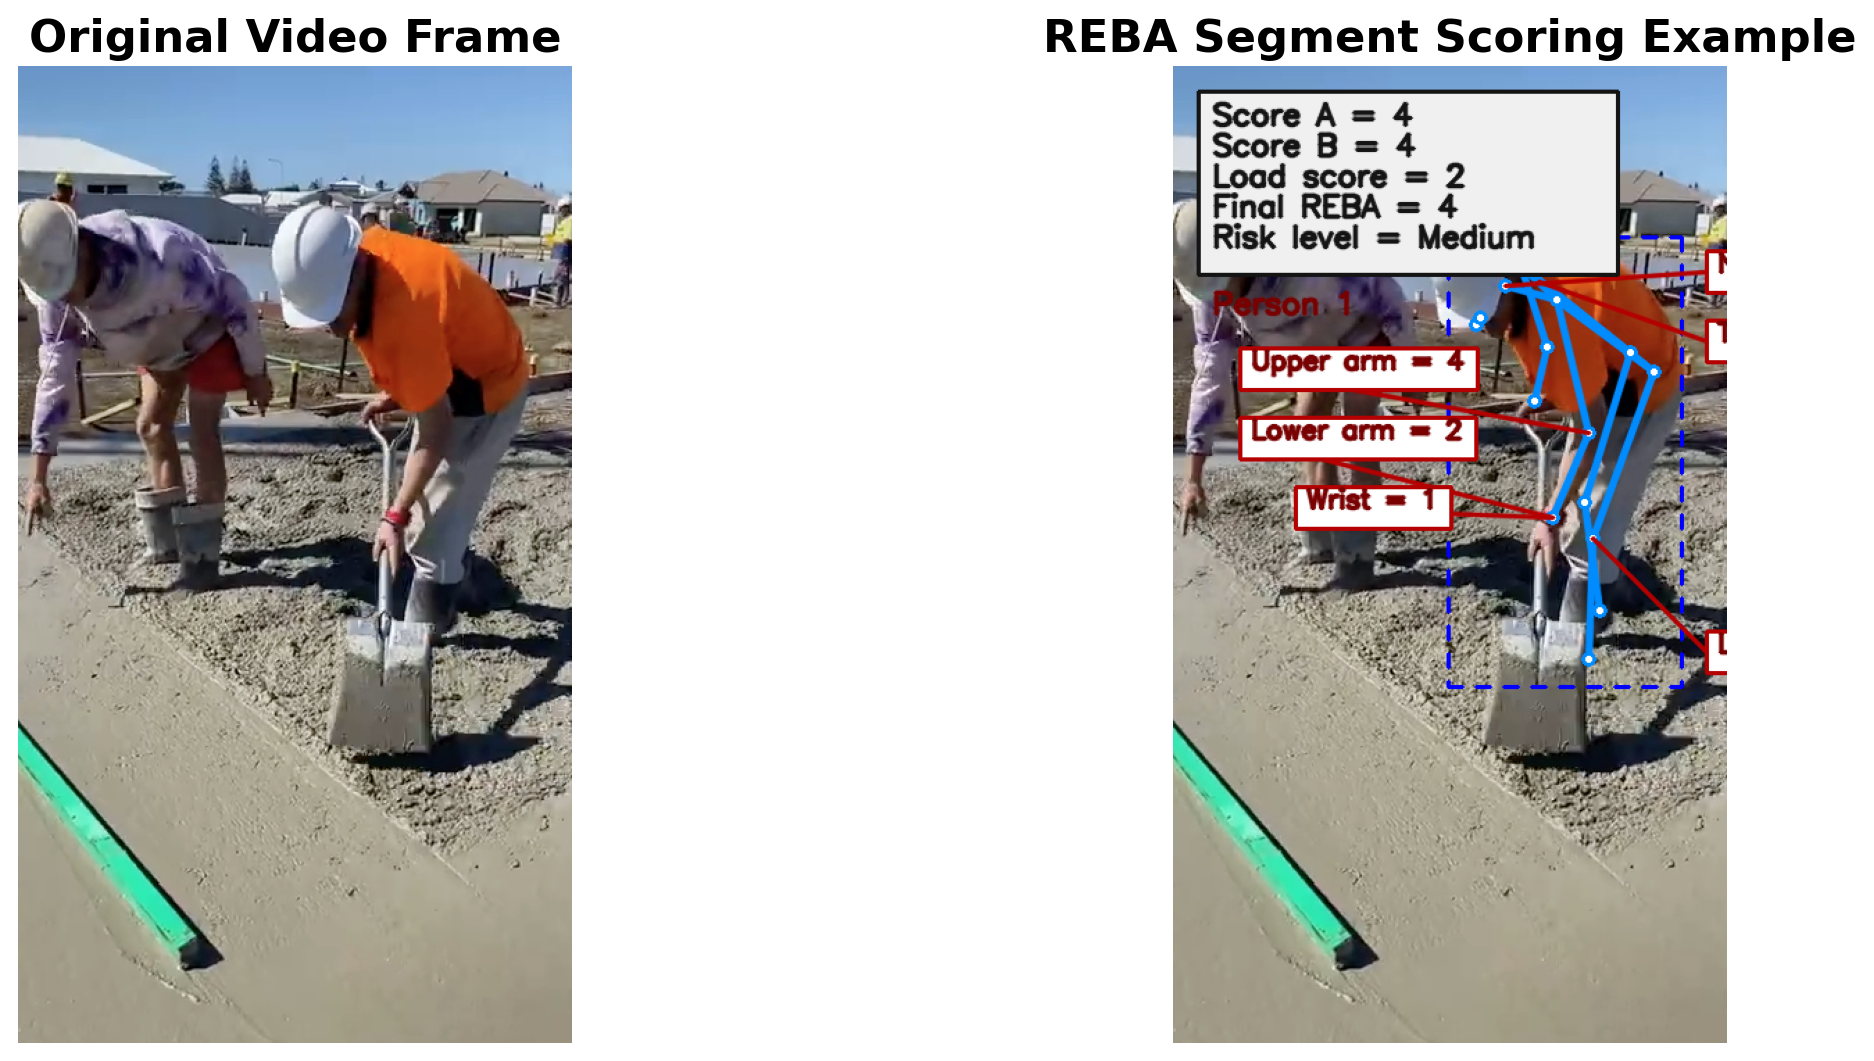
\includegraphics[width=\textwidth]{figures/reba_3.png}
        \caption{Case 3: final REBA score 4 (Medium)}
        \label{fig:reba3}
    \end{subfigure}
    \hfill
    \begin{subfigure}[b]{0.48\textwidth}
        \centering
        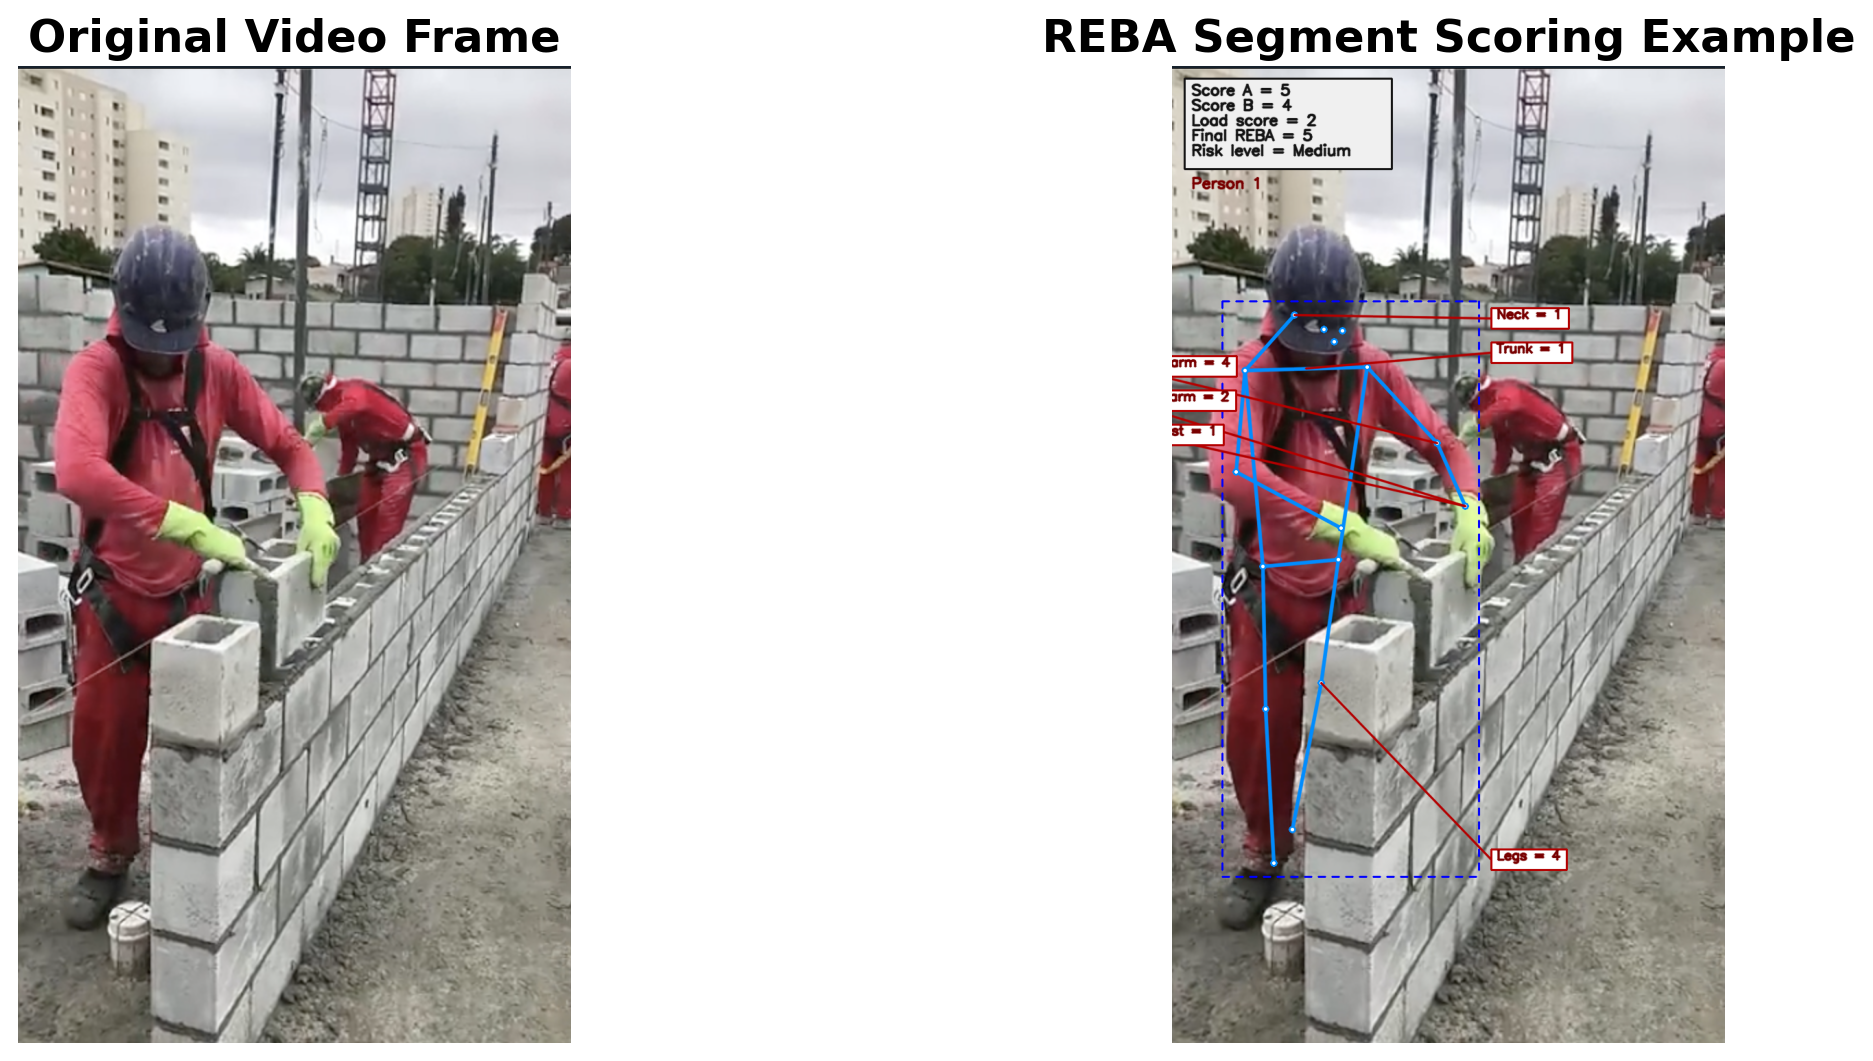
\includegraphics[width=\textwidth]{figures/reba_4.png}
        \caption{Case 4: final REBA score 11 (Very High)}
        \label{fig:reba4}
    \end{subfigure}
    \caption{Full-body REBA scoring examples for Cases 1--4. Each panel shows the original video frame and the corresponding segment-level REBA interpretation.}
    \label{fig:reba_examples_a}
\end{figure}

\begin{figure}[H]
\centering
    \begin{subfigure}[b]{0.7\textwidth}
        \centering
        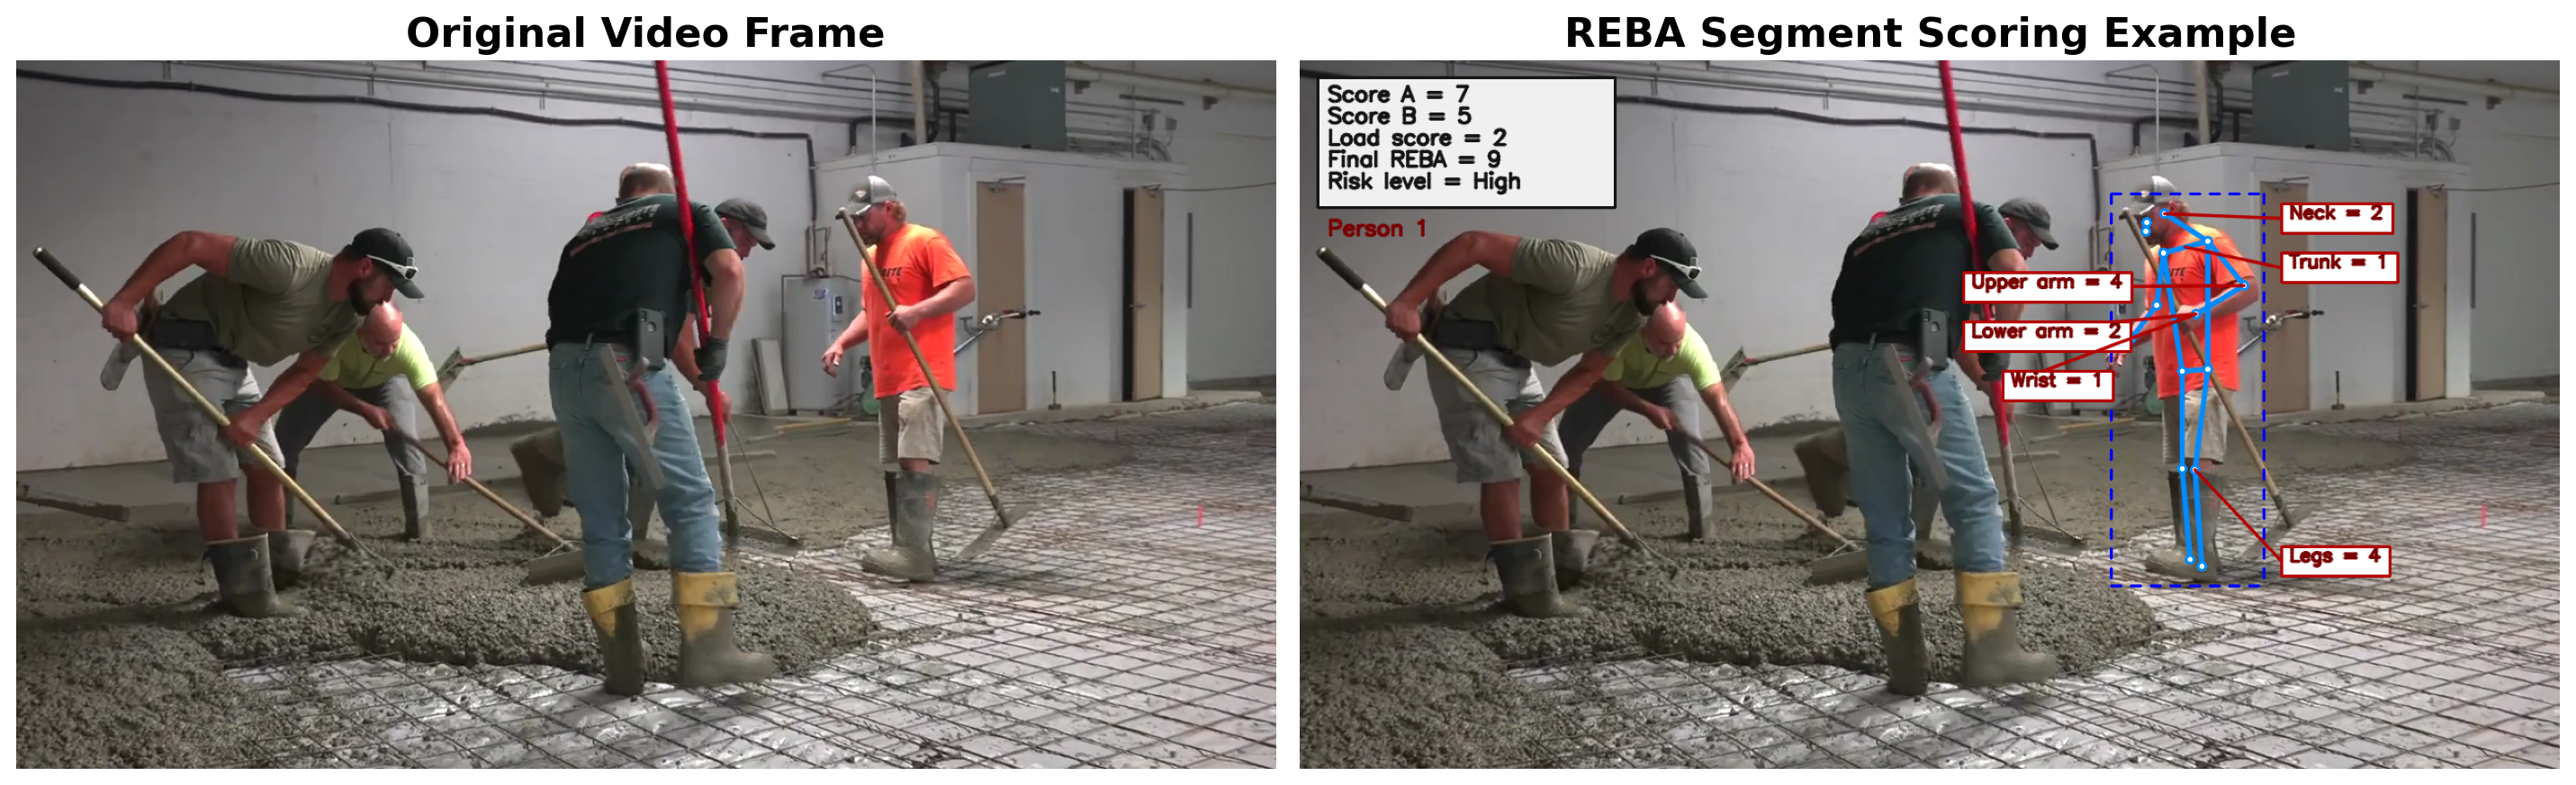
\includegraphics[width=\textwidth]{figures/reba_5.png}
        \caption{Case 5: final REBA score 9 (High)}
        \label{fig:reba5}
    \end{subfigure}
    \caption{Additional full-body REBA scoring example for Case 5.}
    \label{fig:reba_examples_b}
\end{figure}

 \subsection{Benchmark Against Existing Pose Estimation Pipelines}

To provide a direct quantitative comparison with an established baseline, we benchmarked three pose-estimation configurations on five representative clips from the construction dataset: OpenPose, YOLOv8 raw, and YOLOv8 with landmark smoothing. Each clip contained 10 sampled frames, and all methods were evaluated using the same downstream processing pipeline for keypoint filtering,   segment-angle  estimation, bending detection, and  full-body  REBA scoring. The benchmark reports required-keypoint visibility, required-joint coverage, mean and maximum REBA score, REBA standard deviation, mean trunk-angle jitter, proportion of bending frames, and runtime per frame.

Table \ref{table:benchmark_summary} summarizes the aggregate results. YOLOv8 with smoothing achieved the strongest overall balance between pose completeness and temporal stability, with mean required-joint coverage of 71.75\%, mean trunk jitter of 8.69$^\circ$, and runtime of 60.7 ms/frame. In contrast, OpenPose achieved only 46.16\% mean required-joint coverage and 4.0\% required-keypoint visibility, while requiring 2827.3 ms/frame. Compared with YOLOv8 raw, the smoothed YOLOv8 variant reduced trunk-angle jitter from 13.24$^\circ$ to 8.69$^\circ$ while preserving the same keypoint visibility and coverage statistics. These results support the choice of YOLOv8 for the present system and show that the smoothing step improves temporal stability of REBA-related angle estimates without sacrificing throughput.

  Figure \ref{fig:benchmark_cases_grid} presents  all five benchmarked cases in a  compact  3-column layout: OpenPose, YOLOv8 raw, and YOLOv8 with smoothing. Case 1 (drywall clip) shows that both YOLOv8 variants preserve more complete body structure than OpenPose, and smoothing reduces trunk jitter from 15.31$^\circ$ to 13.13$^\circ$ while increasing the mean REBA score from 4.86 to 5.43 by preserving a more pronounced bending posture. Case 2 (hand1 clip) highlights a stronger temporal stabilization effect, where smoothing lowers trunk jitter from 18.32$^\circ$ to 10.08$^\circ$ while keeping the same bending-frame proportion of 60\%; OpenPose detects substantially fewer bending frames at 30\%. Case 3 (kneeling clip) shows the clearest jitter reduction, from 4.08$^\circ$ to 0.13$^\circ$, indicating that smoothing is especially beneficial when posture changes are subtle and the worker remains relatively compact in the image. Case 4 (block clip) shows complete required-keypoint visibility and joint coverage for both YOLOv8 variants, while smoothing lowers trunk jitter from 15.27$^\circ$ to 11.43$^\circ$ and produces a less extreme maximum REBA score than YOLOv8 raw. Case 5 (hand3 clip) is the most difficult of the five examples, with lower coverage for every method; even in this more challenging case, YOLOv8 variants substantially exceed OpenPose in joint coverage. We did not benchmark RTMPose, MMPose, VideoPose3D, or Poserac in the present study, so we do not claim superiority over those methods. Instead, we identify them as important future baselines for broader evaluation, especially for temporal pose refinement and repetitive-action modeling.

\begin{table}[H]
\centering
\scriptsize
\caption{Aggregate benchmark comparison across five construction clips}
\setlength{\tabcolsep}{4pt}
\renewcommand{\arraystretch}{0.95}
  \begin{tabular}{lccccc}
 \toprule
\textbf{Method} &  \textbf{Cov. (\%)} & \textbf{Mean REBA} &  \textbf{Jitter ($^\circ$)} & \textbf{Bend (\%)} & \textbf{Runtime (ms/frame)} \\
\midrule
OpenPose &  46.16 & 4.58 &  20.21 & 32.0 & 2827.3 \\
YOLOv8 raw &  71.75 & 4.67 &  13.24 & 44.0 & 62.05 \\
YOLOv8 + smoothing &  71.75 & 4.78 &  8.69 & 44.0 & 60.7 \\
\bottomrule
\end{tabular}
\label{table:benchmark_summary}
\end{table}

\begin{sidewaysfigure}[p]
 \centering
  \scriptsize
\setlength{\tabcolsep}{4pt}
\renewcommand{\arraystretch}{1.05}
\begin{tabular}{c c c c}
 & \textbf{OpenPose} & \textbf{YOLOv8 raw} & \textbf{YOLOv8 + smoothing} \\
\textbf{\shortstack{Case 1\\Drywall}} &
\includegraphics[width=0.24\textheight,height=0.13\textwidth,keepaspectratio]{benchmark_outputs/best_frames/drywall_clip__OpenPose.png} &
\includegraphics[width=0.24\textheight,height=0.13\textwidth,keepaspectratio]{benchmark_outputs/best_frames/drywall_clip__YOLOv8_raw.png} &
\includegraphics[width=0.24\textheight,height=0.13\textwidth,keepaspectratio]{benchmark_outputs/best_frames/drywall_clip__YOLOv8_plus_smoothing.png} \\
\textbf{\shortstack{Case 2\\Hand 1}} &
\includegraphics[width=0.24\textheight,height=0.13\textwidth,keepaspectratio]{benchmark_outputs/best_frames/hand1_clip__OpenPose.png} &
\includegraphics[width=0.24\textheight,height=0.13\textwidth,keepaspectratio]{benchmark_outputs/best_frames/hand1_clip__YOLOv8_raw.png} &
\includegraphics[width=0.24\textheight,height=0.13\textwidth,keepaspectratio]{benchmark_outputs/best_frames/hand1_clip__YOLOv8_plus_smoothing.png} \\
\textbf{\shortstack{Case 3\\Kneeling}} &
\includegraphics[width=0.24\textheight,height=0.13\textwidth,keepaspectratio]{benchmark_outputs/best_frames/kneeling_clip__OpenPose.png} &
\includegraphics[width=0.24\textheight,height=0.13\textwidth,keepaspectratio]{benchmark_outputs/best_frames/kneeling_clip__YOLOv8_raw.png} &
\includegraphics[width=0.24\textheight,height=0.13\textwidth,keepaspectratio]{benchmark_outputs/best_frames/kneeling_clip__YOLOv8_plus_smoothing.png} \\
\textbf{\shortstack{Case 4\\Block}} &
\includegraphics[width=0.24\textheight,height=0.13\textwidth,keepaspectratio]{benchmark_outputs/best_frames/block_clip__OpenPose.png} &
\includegraphics[width=0.24\textheight,height=0.13\textwidth,keepaspectratio]{benchmark_outputs/best_frames/block_clip__YOLOv8_raw.png} &
\includegraphics[width=0.24\textheight,height=0.13\textwidth,keepaspectratio]{benchmark_outputs/best_frames/block_clip__YOLOv8_plus_smoothing.png} \\
\textbf{\shortstack{Case 5\\Hand 3}} &
\includegraphics[width=0.24\textheight,height=0.13\textwidth,keepaspectratio]{benchmark_outputs/best_frames/hand3_clip__OpenPose.png} &
\includegraphics[width=0.24\textheight,height=0.13\textwidth,keepaspectratio]{benchmark_outputs/best_frames/hand3_clip__YOLOv8_raw.png} &
\includegraphics[width=0.24\textheight,height=0.13\textwidth,keepaspectratio]{benchmark_outputs/best_frames/hand3_clip__YOLOv8_plus_smoothing.png} \\
\end{tabular}
 \caption{  Compact five-case benchmark comparison shown on a single page. Each row corresponds to one clip and each column corresponds to one pose-estimation pipeline evaluated under the same downstream full-body REBA workflow. }
  \label{fig:benchmark_cases_grid}
\end{sidewaysfigure}
 

\DIFdelbeginFL %DIF > DIFDELCMD < \vspace{0.5em}

{%DIF > DIFAUXCMD
}
        %DIF > DIFAUXCMD
{%DIF > DIFAUXCMD
}
        %DIF > DIFAUXCMD
{%DIF > DIFAUXCMD
}
        %DIF > DIFAUXCMD

{%DIF > DIFAUXCMD
}
        %DIF > DIFAUXCMD
{%DIF > DIFAUXCMD
}
        %DIF > DIFAUXCMD
{%DIF > DIFAUXCMD
}
        %DIF > DIFAUXCMD

{%DIF > DIFAUXCMD
}
    %DIF > DIFAUXCMD

{%DIF > DIFAUXCMD
}
        %DIF > DIFAUXCMD
{%DIF > DIFAUXCMD
}
        %DIF > DIFAUXCMD
{%DIF > DIFAUXCMD
}
        %DIF > DIFAUXCMD

{%DIF > DIFAUXCMD
}
        %DIF > DIFAUXCMD
{%DIF > DIFAUXCMD
}
        %DIF > DIFAUXCMD
{%DIF > DIFAUXCMD
}
        %DIF > DIFAUXCMD
{%DIF > DIFAUXCMD
}
    %DIF > DIFAUXCMD

\DIFdelend  \subsection{Recommendations based on VLM-RAG}

Figure~\ref{fig:molmo-result} shows the image of a worker tying rebar at a construction site, along with the prompt and the response generated by Molmo, a vision-language model  \DIFadd{\mbox{%DIFAUXCMD
\citep{deitke2024molmo}}\hskip0pt%DIFAUXCMD
} . The description emphasizes that the worker is adjusting, connecting, and securing the thin metal rods (tying rebar). This detailed account aids the system in understanding the work being performed and serves as an essential input for further ergonomic risk analysis and mitigation strategies. The response from RAG explains that workers can face risks such as poor posture, repeated bending, and awkward movements, all of which can lead to injuries. It offers advice on reducing these risks, such as using better tools and alternating tasks regularly. 

  In the current study, these example recommendations are presented to illustrate the behavior of the VLM--RAG pipeline rather than to claim validated recommendation quality. A systematic evaluation of whether the generated advice is consistently relevant, grounded, and practically effective has not yet been conducted.

  \begin{figure}[H]
    \centering
    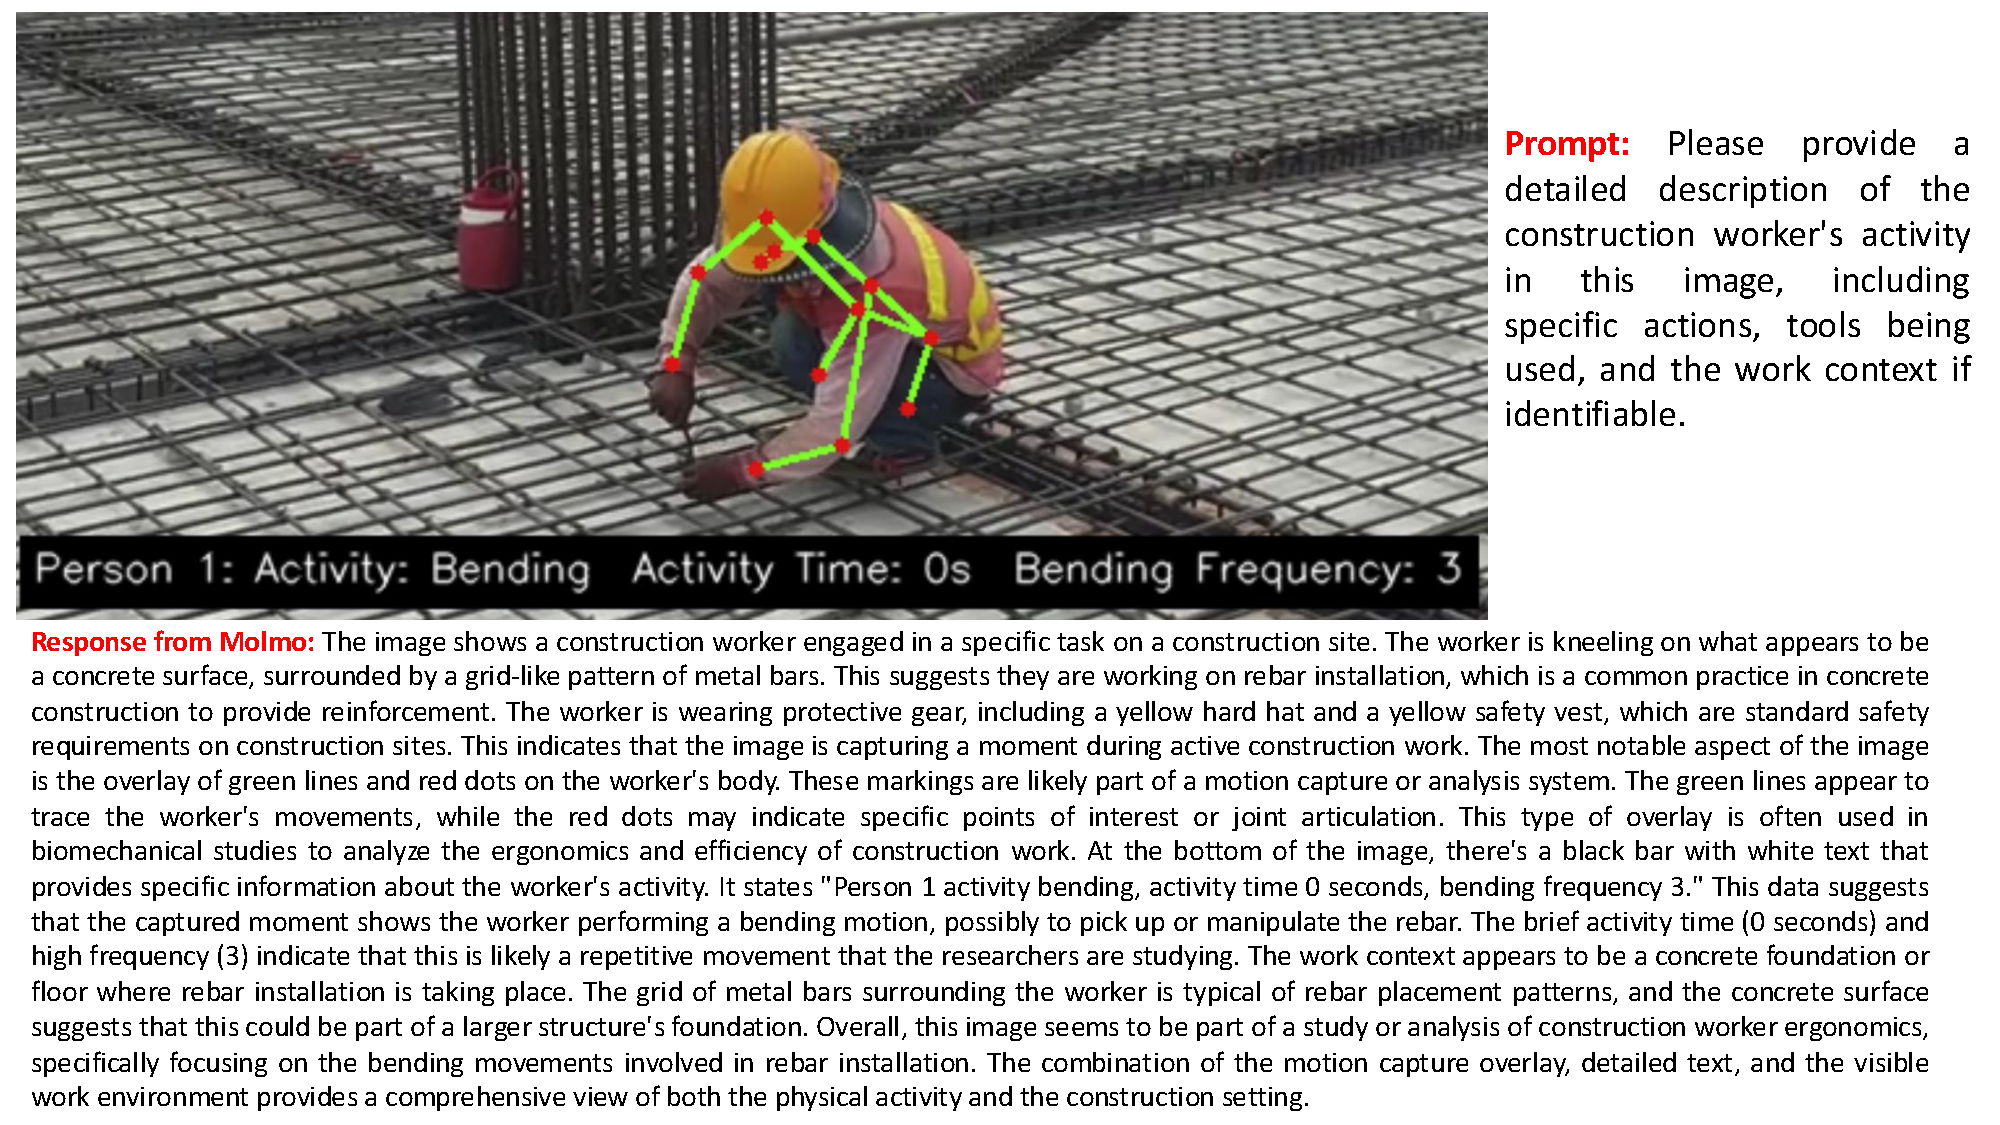
\includegraphics[width=1\linewidth]{figures/Molmo Results.pdf}
    \caption{Response generated by Molmo}
    \label{fig:molmo-result}
\end{figure}

% The RAG part system leverages a collaborative group of specialized agents to effectively answer user questions with accurate references. Initially, the \textit{UserProxyAgent} captures the user's input, initiating the interaction. Subsequently, the \textit{RetrieverAgent} queries a dedicated ChromaDB vector database populated with text derived from safety guidelines documented in \citet{albers2007simple}. This database is structured using embeddings—numerical representations of textual chunks that facilitate rapid and precise semantic comparisons. Once relevant embeddings are identified, the \textit{ContextAgent} compiles and delivers this pertinent information to the \textit{GeneratorAgent}. Utilizing a Large Language Model (LLM) configured at a low temperature setting to ensure consistent and reliable outputs rather than highly creative interpretations, the \textit{GeneratorAgent} synthesizes the retrieved context into a coherent, easy-to-understand response, explicitly citing \citet{albers2007simple}. Finally, the generated response is displayed to the user via a streamlined, user-friendly web interface developed with Streamlit, featuring an intuitive input box for queries and clearly formatted answers.

% The system leverages several helpful libraries to ensure efficient and coordinated functionality. Autogen orchestrates various agents, ensuring each performs its task in the correct sequence. LangChain handles document ingestion, reading and splitting them into manageable segments for analysis. Subsequently, a Hugging Face model generates embeddings, numerical representations of textual data, that are indexed and retrieved efficiently by ChromaDB. With embeddings stored in ChromaDB, the RetrieverAgent can swiftly pinpoint and retrieve document segments most pertinent to user queries. Streamlit facilitates the creation of an intuitive user interface, enabling seamless interaction with the system. Additionally, libraries such as NumPy, scikit-learn, and Matplotlib assist in robust data handling, analysis, and visualization.

% The RAG model starts by using a prompt to gather information, then it retrieves embeddings from that prompt and checks them against the embeddings from \citet{albers2007simple}. This process helps ensure that the image description and other data match the trusted sources.

 

% The simple sentences and detailed explanations provided by the RAG model make it easier for workers and managers to understand the potential hazards and take effective measures. Overall, this approach supports decision-makers in planning safety measures and improving the work environment.

% \begin{figure}[H]
%     \centering
%     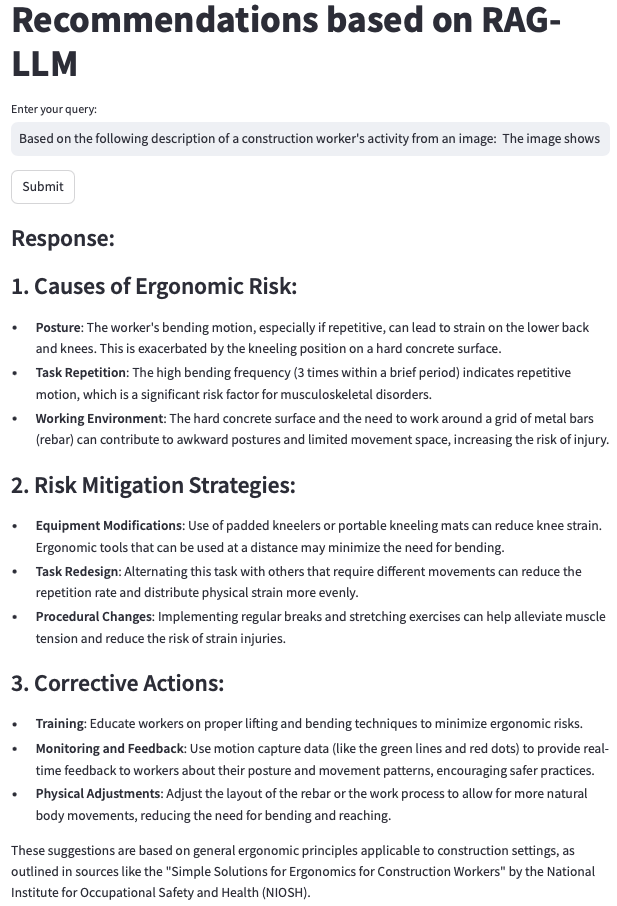
\includegraphics[width=0.5\linewidth]{figures/RAG-LLM Recommendations.png}
%     \caption{Recommendations based on RAG-LLM}
%     \label{fig:rag-llm-recommendations}
% \end{figure}

\section{Conclusion}

The proposed real-time ergonomic risk detection system is able to     identify and assess   construction workers' postures   from ordinary video  . The results demonstrate the system's capability to track bending and standing postures, measure activity duration,     count posture transitions, and compute a full-body REBA score from YOLO pose keypoints. The revised workflow evaluates neck, trunk, upper-limb, wrist, and leg postures, combines them through REBA Tables A, B, and C, and incorporates a VLM-assisted approximate load/force estimate to assign the final risk level. Landmark smoothing improves temporal stability of the detected keypoints, and the benchmark shows that the YOLOv8-based pipeline provides a much stronger balance of speed and pose completeness than OpenPose on the five representative construction clips .  By providing real-time feedback, the system enables safety managers to proactively identify and mitigate ergonomic risks.     A notable advantage of the proposed system is its cost-effectiveness and accessibility. Unlike traditional ergonomic assessment methods that often require expensive specialized equipment, this system can be implemented using standard hardware, a regular     commercial-grade camera,   and a computer with moderate processing capabilities.

% Additionally, most prior studies emphasize posture classification without continuously measuring the duration of bending postures, a key factor in musculoskeletal risk assessment. 

% By incorporating real-time feedback and continuous monitoring, the proposed system overcomes these limitations and provides a more comprehensive assessment of ergonomic risks in construction settings.

% The observed results can be attributed to the efficiency of YOLOv8 in detecting human poses and the effectiveness of landmark smoothing in refining posture analysis. The high accuracy in detecting bending activities is likely due to the system's ability to track key joint landmarks. This allows for precise calculation of trunk angles. The slight discrepancies between model predictions and manual evaluations can be explained by occlusion effects, variations in camera angles, and challenges in distinguishing borderline postures. Additionally, environmental factors, such as poor lighting or dynamic worker movements, may have influenced detection accuracy.

% The findings have several implications for improving workplace safety in the construction industry. 

% This approach aligns with industry trends toward using AI-driven solutions to enhance worker safety and productivity.

Despite its effectiveness, the system has some limitations. The accuracy of pose detection may decrease in cases where workers' movements are partially occluded or when multiple workers overlap in the camera’s field of view.   In addition, posture duration may be underestimated when a worker moves out of frame because the current activity segment is closed at the last valid detection and any later reappearance is treated as a new segment. Another important limitation is that trunk  and limb \DIFadd{ angles are computed from 2D projections of body keypoints obtained from a single camera. When the worker's torso is rotated relative to the camera plane, the projected 2D angle may deviate from the true 3D  flexion angle, which can in turn affect REBA-related interpretation. This limitation is consistent with prior evidence that joint-angle estimates derived from 2D and 3D camera measurements can differ meaningfully depending on viewpoint and measurement setup \mbox{%DIFAUXCMD
\citep{vancrombrugge2022accuracy}}\hskip0pt%DIFAUXCMD
.   }The load/force term is also estimated approximately from the object or tool category inferred by the VLM rather than from direct physical measurement, so the assigned load score should be interpreted as a practical approximation. A further limitation is that the VLM--RAG recommendation module has not yet been evaluated by domain experts and has not been systematically validated through user studies, inter-rater agreement analysis, or task-level outcome measures. As a result, the current manuscript cannot claim that the generated recommendations consistently improve worker behavior or reduce ergonomic risk in practice .  Future improvements could involve refining the detection algorithm to handle more complex postures  , incorporating 3D pose reconstruction or multi-camera capture,   validating the VLM-assisted load estimates against measured weights, and conducting formal evaluations of recommendation quality using groundedness, relevance, actionability, usefulness, and human-subject feedback metrics  . Future research should   also   focus on enhancing the system’s real-time feedback mechanisms by incorporating predictive analytics to identify workers at risk before injuries occur. Additionally, integrating multimodal data, such as wearable sensor inputs and physiological indicators, could improve the system’s accuracy in assessing ergonomic strain.

% Furthermore, the utilization of open-source software components, including the YOLOv8 model, significantly reduces implementation costs. This economic feasibility makes the technology particularly attractive for small and medium-sized construction contractors who may have limited resources for safety monitoring systems. The low cost barrier to entry could encourage wider adoption of automated ergonomic risk assessment across the construction industry, potentially improving worker safety outcomes across projects of all sizes.

% The proposed real-time ergonomic hazard detection system aims to reduce musculoskeletal risks among construction workers by using the latest pose estimation method. This study demonstrates that real-time posture tracking and activity duration measurement can effectively identify hazardous postures and provide immediate feedback to workers and supervisors. The evaluation results indicate that the system is able to successfully detects ergonomically risky activities with high accuracy. 

% This research contributes to the broader field of construction safety by offering a scalable and non-intrusive ergonomic assessments. By integrating real-time feedback mechanisms, the system has the potential to enhance workplace safety and worker well-being, which will ultimately improve productivity and reduce injury-related downtime. The findings emphasize the importance of continuous posture monitoring in addressing ergonomic risks, particularly in dynamic construction settings.

% The study has practical implications for construction site management, as it provides an automated tool for real-time ergonomic assessment. The system, which has the ability to track postures and alert supervisors to risky behaviors, enables proactive interventions. This helps in reducing the likelihood of work-related musculoskeletal disorders. Theoretically, this research advances the application of computer vision in occupational safety by demonstrating how pose estimation models can be adapted for ergonomic risk detection in complex work environments.

% Future research should focus on deploying the system in live construction environments, where it can be evaluated for its performance under real-world conditions. Expanding the system’s capabilities, so that it can track additional ergonomic risk factors, such as repetitive motion and force exertion, could further enhance its effectiveness. The integration of wearable sensors, which will allow physiological monitoring, and the development of predictive models based on historical data will provide deeper insights into worker safety. Collaboration with industry stakeholders will be essential, as it will help refine the system for practical implementation and encourage widespread adoption.

\bibliographystyle{unsrtnat}
\bibliography{ref}

\end{document}
